\documentclass[12pt,%
               %draft,%
               a4paper]{uiothesis}

\usepackage{graphicx}
\usepackage{longtable}
\usepackage{lscape}
\usepackage{natbib}
\usepackage{paralist}
\usepackage{ragged2e}

\title{Social Navigation on the Social Web}
\subtitle{Unintrusive Prototyping in Established Spaces}
\author{Eivind Uggedal}

\includeonly{%
%acknowledgements,%
%introduction,%
%background,%
%methodology,%
%analysis,%
selection.of.third.party.software,%
implementation,%
%discussion,%
%conclusion,%
%content.inventory,%
%source.code,%
}

\begin{document}
  \chapterstyle{uio}
  \pagestyle{uio}
  \maxsecnumdepth{subsubsection}

  \frontmatter
    \pagenumbering{alph}
    \maketitle
    \pagenumbering{roman}
    \cleardoublepage
    \tableofcontents
    \cleardoublepage
    \listoffigures
    \cleardoublepage
    \listoftables
    \cleardoublepage
    \listofsourcecode
    \chapter{Acknowledgements}

Asbj\o{}rn F\o{}lstad at \abbr{SINTEF} was of great help in building the
research design used for real world user testing and accepting our work as
part of the \abbr{RECORD} project where we were able to obtain founding.
Morten Skogly at \abbr{NRK},
urort{} was helpfull with providing information about their web site and
recruiting users for testing our navigational prototype.

I'd like to thank
Andreas Dieberger,
Peter Brusilovsky, and
Robert Mer\-t\-ens
for allowing me to freely use illustrations from
some of their published articles.

Last but not least I'd like to thank my supervisor, Gisle Hannemyr, for
his guideance and thoughtfull input during the whole master thesis process.


  \mainmatter
    \chapter{Introduction}
\label{chapter:introduction}

The web has come a long way since its inception when it functioned as a
global interconnected system for document sharing amongst researchers
\citep[\p{82}]{bernerslee92}. We've
seen the coming of an increasingly more social web as
\postquote[\p{44}]{backstrom06}{%
  the digital domain has seen a significant growth in the scale and richness
  of on-line communities}
There have been
an increase from 18\% to 45\%
\begin{sparkline}{3}
  %Name  Size Unit
  %2005  16%  .356
  %2007  45%  1
  \sparkspike .25  .356
  \sparkspike .75  1
\end{sparkline}
in blog usage by the general public%
\sidenote{%
  Represented with a total of 6,545 respondents
  to a survey conducted in Canada, France, Germany, Japan,
  the United Kingdom, and the United States
  by \citet[ch.~1, \p{2}]{rosa07}.
}
in an 18 month period from 2005 to 2007.
It has been argued that web citizens'
familiarity with blogging laid the groundwork for the explosion we are seeing
in user participation in web communities
\citedouble{\p{20}}{weiss05}{\para{2.2}}{beer07}.

At the same time advances in hardware and web development tools have made it
easier and cheaper to create new web sites. We're now seeing an
abundance of new offerings in this field.
It has been argued that many of the concepts this modern web brings are
evolutionary instead of revolutionary \citep[\p{45}]{yakovlev07}.
\citet[\p{17}]{treese06} also witnesses a continuous evolution, but with
exploratory innovations as he notes that most technological changes are
incremental.%
\sidenote[-4]{
  \prequote{knuth07}{%
    also believes innovation in computer science is incremental:}{%
      I firmly believe that computer science advances by thousands of people
      solving small problems, which go together and create a massive edifice.
      Every year that goes by, hardly anything is done that appears to be a
      milestone worthy of mass attention; yet after five or ten years pass,
      the whole field has changed significantly}
}
\begin{fullquote}[\p{18}]{weiss05}{have seen this trend}
  When we consider a hot, buzz-worthy Web site of the new Internet evolution
  [\ldots]
  they are at the same time incredibly innovative and yet\dash{}not.
\end{fullquote}

What we're experiencing
today with the World Wide Web and social/collaborative software systems was
envisioned several decades ago by \citet{licklider68} and \citet{bush45}.

During the initial studies of our research we frequented
many of the these modern web sites. Our impression is that
this area of the web infamously coined \term{Web 2.0}\dash{}an
increment in version opposed to the age when the Web was in its
infancy\dash{}is bringing interesting innovations. While they might not be
groundbreaking, we justify a closer look at them in this thesis.

\section{Focus}

This thesis have a focus on navigational problems and only those
which are of a social type.%
\sidenote{%
  Take a look at \sectionref{social.navigation.social.navigation}
  to learn more about navigational systems with social characteristics.
}
Navigation in context of computer systems is
essentially a metaphor based on how people find their way in the physical
world. So just as a compass and map can be crucial in your ability to find a
cabin deep in the woods during a hike\dash{}reliable and efficient
navigational systems on the web is of uttermost importance when you're trying
to locate a certain electronic object containing valuable information.

In addition to only focusing on \term{social navigation} we're only concerned
which such types of navigation on the Web.
On the Web we're using hyperlinks \citep[\p{90}]{nelson65} to provide users
with navigational choices. We're only focusing on the use of such hyperlinks
within web browsers and not navigation support in auxiliary tools as email
clients, instant messaging clients, and so on. Our focus is further refined by
targeting our research  only on what happens inside various web pages. This
means that other navigation forms supported by the browser itself or third
party extensions or plugins is outside of our scope, as detailed in
\sectionref{social.navigation.navigation.navigation.on.the.web}.

While we're aware that search is an important part of peoples every day
navigational behavior we've introduced additional confinements and decided to
only concentrate on browsing behavior (see
\sectionref{social.navigation.navigation.navigation.on.the.web} for details).

When studying various web pages it became apparent that some use of
social navigation mechanisms implies pretty large privacy concerns. By mining
users' previous actions specific user profiles can be generated. One can then
represent very sensitive characteristics of individuals such as sexual
orientation, political status, and religious beliefs.
We feel this subject area of social navigation in relation to privacy warrants
a master thesis on its own. Discussion of privacy concerns have therefore
been excluded from our research so that we can look more closely at the
navigational characteristics of social navigation.

\section{Motivation}

\sidetable[Social Navigation in Academia]{%
           Social navigation in academia, by content
           \label{table:social.navigation.academia}}{%
  \begin{tabular}{lr}

    & Articles \\

    \cmidrule(lr){2-2}

    Modern Web & 5 \\
    Other & 21 \\

  \end{tabular}
}

Social navigation are as we'll see in
\sectionref{social.navigation.social.navigation}
a well defined term within the academic community.
During our literature review we collected to the best of our abilities all
academic articles where social navigation was discussed. Our approach was to
use keyword search and citation search in the databases listed in
\tablepageref{literature.databases}.%
\sidenote[2]{
  For more about our literature collection method, see
  \sectionref{literature.search}.
}
\tableref{social.navigation.academia} shows the metrics of articles
we found about social navigation in context of the modern web as captured by
the Web 2.0 term (social network sites, folksonomies, and wikis) and other
areas of computer science (classic web, general user interfaces, security, and
so on).
On several occasions we encountered similar articles by the same authors
discussing the same problems and systems. In such circumstances the collection
of two or more similar articles was counted as one.

Our current area of Web 2.0 in relation to navigational problems have in our
view (based on our literature findings) little coverage in academia.
\prequote{beer07}{notes that}{%
 \,`internet time' now runs at at a clock speed several orders
 of magnitude faster than that of academic research}
We described earlier the growth we're seeing of web sites with social
aspects and we believe that some of these provide for novel examples of social
navigation. It would therefore be interesting to look at some of the
state-of-the-art social web sites and look at what contributions they have
made to the field of social navigation.

We are currently lacking information on how one can use social navigation
consciously in a modern web application design process. Such navigational
schemes seem to be created without guidance and many times as an afterthought.
It appears that methods for establishing incentives for user participation
is the focal point of web architecture design today. Even though such
approaches can result in sound and interesting navigation it's our impression
that a focus on solving users' navigational problems is more beneficial for
the usability of a web site. We try to take such an approach when we design a
navigational prototype (see \sectionref{implementation.design} for details).

\section{Objective}

By collecting examples of good navigational implementations in the wild
and analyzing them we hope to give a clearer
view of the field of social navigation in our modern web.
As we are unaware of any established technique for
conducting such a study on real world navigation systems we create our own
method as we go\dash{}fine tuning it as we learn from our experiences.

Using the knowledge we gained from collecting social navigation examples
from real world web sites we try to improve an existing web site by
implementing a navigational prototype. The navigational technique we
decided on implementing is a so called \term{activity stream}. See
\sectionref{analysis.facebook.news.feed} and
\sectionref{implementation.design.activity.stream}
for more information about this particular navigational technique.

The Norwegian Broadcasting Corporation's joint
\abbr{TV}, radio, and internet project \project{\urort{}}\dash{}a site where
artists upload their demos and get valuable playtime on radio and \abbr{TV} if
their products are judged to be of sufficient quality\dash{}was
the candidate for implementing a navigational prototype.
Our focus was on the \urort{} web community%
\sidenote{
  Available at \url{http://nrk.no/urort}.
}
where users can interact in a social manner, listen to other people's songs,
and upload their own creations.
We decided to build our application in an transparent manner on top of the
web site \urort{} offered. The rationale for such a decision can be found in
\sectionref{implementation.building.on.top.of.the.web}.

With our technical solution in place we were able to test how it performed in
practice by conducting an empirical experiment with real world users.

\section{Contributions}

Contributions from our research on social navigation is threefold:

\begin{enum}
  \item Informing navigational design by giving a structured overview of
    various social navigational schemes used in academia and the real world.
  \item Exemplifying transparent prototyping methods by sharing experiences
    with creating an unobtrusive shell of navigational designs on top of an
    existing web site.
  \item Applicability of a particular social navigation technique
    by discussing findings from an experiment of its real world usage.
\end{enum}

\section{Outline}

This thesis is composed of two parts:

\begin{enum}
  \iterm{Social Navigation on the Social Web}. In this part we first give you
    background information about social navigation before
    we analyze social navigation in two modern social web sites.
  \iterm{Unintrusive Prototype of Social Navigation}. The second part starts
    with an account of how we created an unintrusive social navigation
    prototype before we go through an empirical study of the prototype
    implementation.
\end{enum}

After these two parts we conclude our work and give pointers to future work
in \chapterref{conclusion}.

    \chapter{Background}
\label{chapter:background}

% 1. how the literature was collected (describe it pragmatically)
%
% 2. literature review (summary, analysis, and comparisons)
%
%   A literature review should answer:
%
%     * What do we already know about the topic?
%     * What do you have to say critically about what is already known?
%     * Has anyone else done anything exactly the same?
%     * Has anyone else done anything that is related?
%     * Where does your work fit in with what is done before?
%     * Why is your research worth doing in the light of what has
%       already been done?
%
%   A literature review should be a dialogic rather than a mere
%   replication of other peoples writing. Should not be a laundry
%   list of previous studies.
%
%   Be focused and critical. Include an incisive critique that will help your
%   peers see the world differently.
%
% 3. introduction to terms as folksonomy, tagging, geotagging, etc
%
% 4. paragraph or two about my subject related to popular literature
%    (search Amazon or Library of Congress and say something like: there
%    were X books about this subject, the first was published in 2001
%    but the majority of books were published the last two years, and
%    maybe show a graph)

\section{Literature Search}

Before a literature search was conducted we did some preliminary thinking
about
\begin{inparaenum}[(i)]
  \item the focus of our topic to get more precise results, and
  \item what literature databases would yield sufficient and accurate
    findings.
\end{inparaenum}
Based on these concerns we settled on the literature indexes laid out in
\tableref{literature.databases} and used the following keywords%
\sidenote{
  With varying use of modifiers (i.e. AND) or quotations to find exact phrases
}
for search:

\begin{description}
  \item[social navigation] is the concept of our main topic.
  \item[collaborative filtering] is often used to realize our main topic.
  \item[recommender system] can be an application of our main topic.
  \item[tagging] can be related to our topic depending on use.
\end{description}

\begin{table}
  \centering
  \caption{Literature Databases}
  \label{table:literature.databases}

  \begin{tabular}{p{20pc}l}

    \toprule
    Name & Type \\
    \midrule

    ACM Digital Library &
    Full-text \\

    The Collection of Computer Science Bibliographies &
    Bibliography \\

    Inspec Online &
    Reference \\

    HCI Bibliography &
    Bibliography \\

  \end{tabular}
\end{table}

In addition to keyword based search we also conducted citation searches on the
articles that in our opinion seemed to be the most important in the field.
The articles that we found relevant during our literature search phase was
collected and studied. During this process we eliminated articles by the same
authors where similar topics and implementations were discussed and focused on
either the most recent or the most representative article.

First we'll briefly discuss navigation and sociality both in general terms
and relating to the web. Then we'll concentrate on these two topics together
by looking at the research where social navigation is used
consciously as a concept. By this we mean the research where either social
navigation is defined, redefined or problems relating to the concept is
discussed with a basis in such definitions.
After our main survey of social navigation research we'll look at topics
which we believe can be included in the discussion of social navigation or are
closely related.

Some of the research that has been conducted in the space of
social navigation and related areas does not share our focus on the Web.
We still found much such research interesting in spite of their attention to
generalized problems or specific problems in other fields than the Web.

\section{Navigation}
% Try to cite some classic work. First navigation systems

Navigation was traditionally associated with controlling a weasel at sea to
a given destination.%
\sidenote{
  \emph{Navigate} is in fact derived from the two Latin words \emph{navis}
  meaning ``ship'' and \emph{agere} meaning ``to drive''.
  \citep[p.~756]{anderson97}
}
Since then it's been used to describe behavior related to safely finding ones
way whether one is driving a car, flying a plane or walking on foot. Maps
(a graphical representation of the medium one are navigating in)
and compass (a tool for connecting graphical maps to the physical world)
are often used as aids in this way finding. When used in context of
computer systems navigation is essentially a metaphor of our usage of the
word in our physical world. Trough computer systems we present users with a
conceptual space in wich they can navigate \citep[p.~189]{whiteside85}.

\subsection{Navigation on the Web}

\citet{jones96} studied the navigational support provided by the Web's first
browsers:
\begin{inparaenum}[(i)]
  \item loading of page by entering it's location,
  \item loading a bookmarked page,
  \item loading a page by using a hyperlink on the current page,
  \item recall previously visited pages with forward and backward buttons,
  \item recall a previously visited page by locating it in a history list, and
  \item reloading the current page.
\end{inparaenum}
While modern web browsers support more forms of navigation%
\sidenote[-8\onelineskip]{
  These early browsers' history lists were not remembered between sessions. In
  addition we're seeing browsers as Flock (available at
  \url{http://flock.com}) with new methods of navigation integrated and also
  an abundance of plugins and extensions for the main stream browsers that
  enable new possibilities for navigation.
}
than the earliest applications we're not concerned with those here.
We're only interested in the navigation which are conducted within the main
browser window (where web pages are rendered) enabled by following hyperlinks.

\section{Sociality}

The Oxford English Dictionary, second edition \citep[p.~905]{simpson89}
defines the adjective \emph{social} as:

\begin{quote}
  Capable of being associated or united \emph{to} others.
\end{quote}

Discussion about explicit social matters is left for scholars of the social
sciences. We've therefore briefly introduced the term and are more concerned
with situations where it's related to computer systems, and most importantly:
the Web.

\subsection{Sociality on the Web}
% Discuss sociality on the web. Maybe a good place for a Web 2.0 discussion.

Sociality has become an integral part of our modern web.
\citeauthor{bernerslee07}, seen by many as the inventor of the Web,
recently discussed the evolution from the Net (III: International
Information Infrastructure), trough the Web (WWW: World Wide Web),
to what he calls \emph{the Graph} (GGG: Giant Global Graph) in a
blog post \citeyearpar{bernerslee07}. The Graph is synonymous with the
\emph{Semantic Web}%
\sidenote{
  The Semantic Web is a web where data and information can be meaningful
  to computers and not just humans \citep{bernerslee01}. Altough this idea was
  introduced by \citeauthor{bernerslee07} in 1994 it reamins largely
  unrealized to this day \citep[p.~96]{shadbolt06}.
}
and he describe it in relation to
current trends of sociality on the Web:
\begin{quote}
  It's not the Social Network \emph{Sites} that are interesting--it is the
  Social Network itself. The Social Graph. \citep{bernerslee01}
\end{quote}

In other terms this means that social relationships on the Web have become so
important that they're more interesting themselves than the pages that
represents them.

\subsubsection{Web 2.0}
% tie in definition from oreilly in introduction chapter.
% cite web 2.0 general papers
% cite weiss05 paper, collective intelligence
% self sufficient user base
% need early adopters, not imediate benefit before the user base is sufficient
% large. term for this, can't remember the name

\section{Social Navigation}
\label{section:background.social.navigation}
Drawing on the previous explanation of navigation and definition of social, we
can combine the two terms. Social navigation then means going from one point
to another in a medium with other people.

Social navigation as a term was introduced in a short article by
\citet{dourish94} where they discussed three types of navigational mechanisms,
spatial, semantic, and social, which they argue can be separated even though
there is evidence of situations where the different mechanisms are combined.
In their description of the social type they coined the term
\emph{social navigation}:

\begin{quote}
  When navigable information systems are extended to support collaborative
  activity, a third model of navigation arises. This is \emph{social}
  navigation. In social navigation, movement from one item to another is
  provoked as an artifact of the activity of another or a group of others.
  \citep[p.~1]{dourish94}
\end{quote}

\citeauthor{dourish94} exemplifies two cases where neither location
(spatial) nor content (semantic) is used for exploration--the social model
is used on it's own. The first example is of home pages where the creators
have authored a list of web pages they find interesting. Their second example
is of the Tapestry \citep{goldberg92} system where electronic messages can be
voted upon and users can use such metrics for navigating items that seem to be
of interest. Such a technique is called \emph{collaborative filtering},
a term which will be discussed later as a concept enabeling social
navigation. Based on these two experiences \citeauthor{dourish94} argues that
we possibly need to move away from spatial models of navigation and rather
focus on designing explicitly with semantic and social navigational
techniques.

\citet{dieberger97} introduced a more throughout review of social navigation
on the Web. \citeauthor{dieberger97} builds on the ideas introduced by
\citeauthor{dourish94} and looks at it from a more practical standpoint when
he describes navigational behavior on the Web in it's earlier days, the state
of social navigation support in the tools of the time, and review two
prototype systems with social navigation features.

\subsection{Hyperlink Sharing}
% favorite bookmarks on home pages, feel that it's seen now as blog-rolls
% social bookmarking, leads to next subsection
% delicious, lot of more, some academica related like citeulike and so on
% stumbleupon

Both \cite{dourish94} and \cite{dieberger97} observed social navigation on the
Web when hyperlinks were shared on web pages. Creators of these pages often
had a list of pointers to other web pages they deemed interesting enough to go
trough the trouble of creating such a listing. By doing this they created
an opportunity for navigation based on social factors.
\citeauthor{dieberger97} calls this form of hyperlink sharing passive
based on the nature of the exchange between the two parties--the creator and
the reader. He goes on an distinguishes passive sharing from an active
approach where a person either deliberatly seeks out another and asks for a
pointer or intentionally gives a pointer away.


\subsection{Item Annotation}
% tagging
% articles with tagging in context of social navigation
% lot of more discussion of tagging and mostly related to organizing
% principles and folksonomy

\subsection{Hyperlink Trails}
% bush, wexelblat99, new services, trailfire, new hoodwink.d greasemonkey
% service

\subsection{Collaborative Filtering}
% introduce earlier cited goldberg92 article and more recent work. recommender
% systems ties into this

\subsection{Off the Web}
% security, mathematical models, etc

\subsection{Visualization}
% activity, usage, edit/read wear

\section{Building on Top of the Web}
% greasemonkey, hoodwink.d, new hoodwink.d service
% browser extensions related, greasemonkey itself a extension, but
% thinking about specialized plugins for enabeling interaction on top of other
% web pages.
% mashups kind of related, maybe put inside web2.0 part or seperate part
% open apis is the fuel for mashups. possible without by screen sraping, but
% not as convenient and safe (upgrades on the pages we're scraping)
% facebook, open social. apps on top of social network sites. installed base
% of users and relationships already in place.

\section{Summary}

Based on our discussion of secondary background literature we've introduced
several terms:

\begin{description}
  \item[Web 2.0]
  \item[Social navigation]
  \item[Collaborative filtering]
  \item[Tagging]
  \item[More to come]
\end{description}

    \chapter{Methodology}
\label{chapter:methodology}

This chapter will include information in how data was collected. So far this
includes content inventory/analysis.

\section{Content Analysis}

The term \term{content analysis} is traditionally used to signify a
qualitative research method used in the social sciences.
\prequote[\p{18}]{krippendorff03}{defines it as}{%
  a research technique for making replicable and valid
  inferences from texts (or other meaningful matter) to the contexts of their
  use}
Even though such an analysis of the contents, meanings, or effects of
communication messages also have been utilized on the Web \citep{weare00}
it does not seem very well suited for understanding navigational mechanisms.

We turn to content analysis as the more pragmatic practice conducted within
the field of \term{information architecture}%
\sidenote{
  Information architecture can be explained as
  \begin{inparaenum}[(i)]
    \item the structural design of shared information environments,
    \item the combination of organization, labeling, search, and navigation
      systems within web sites and intranets,
    \item the art and science of shaping information products and experiences
      to support usability and findability, and
    \item an emerging discipline and community of practice focused on bringing
      principles of design and architecture to the digital landscape
      \citep[\p{4}]{morville06}.
  \end{inparaenum}
} hoping that it will help us get an better understanding of navigational
structures.
Content analysis is deployed as a technique by information architects for
helping them generate a sound and well structured web site architecture.
It's seen as a bottom-up process and
in its essence a content analysis should identify the various
relationships (or lack of correlation) between a web site's content items.
It consists of two phases:
\begin{inparaenum}[(i)]
  \item a collection of a representative sample of data and
  \item an analysis of this collected data
\end{inparaenum}
\citep[\pp{241}{243}]{morville06}.

Information architects are concerned with
the system's content and
\postquote[\p{94}]{batley07}{%
  need to move below the surface of the system
  interface to examine the system information itself}
We on the other hand are actually concerned with the system interface and
specifically its navigational structures. This creates a striking
contradiction as we're not interested in content unless it can help or
guide users during their navigation. We therefore have to adapt
both our inventory and analysis process accordingly.

\subsection{Inventory}

A \term{content inventory} is a technique for collecting data from web sites
in a structured manner. It's strength as a technique lies in its ability of
truly informing about a web site's content \citep{wodtke02}. The process of
actually conducting a content inventory can be equally rewarding as the
resulting documents \citep{veen02}.

\subsubsection{Sampling}
\label{section:methodology.content.analysis.sampling}

Content inventories are often tedious and time consuming to perform.
\citet[\p{267}]{wodtke02} argues that every single bit of content needs to be
determined while \citet[\p{241}]{morville06} believes a representative sample
is sufficient.

The web sites that are interesting to look at in our research are vast and
loaded with enormous amounts of user generated content. An all-inclusive
approach to content gathering would simply be impossible in such situations.
As a remedy to this we've decided to ignore certain parts of web sites in our
content inventories since the scope of our research is limited to navigational
constructs and only those which have a social nature.

Our experience is that social navigation and more static navigation are
intermixed all over web sites. Often one have to use non-social forms of
navigation before social navigational options appear. Thus we could not simply
ignore navigational aims which were non-social in our content inventory phase.
We did however eliminate the following parts of web sites under investigation:

\begin{enum}
  \iterm{Administrative sections} where users can change their profiles or set
    their preferences.
  \iterm{Help pages} where \abbr{FAQ}s, guides, and instructions are presented
    in a static manner.
  \iterm{Legal information} including terms of service, privacy policies, and
    copyright notices.
  \iterm{Content generation} facilities like uploading, categorizing, and
    editing photos, commenting, posting items, and so on%
    \sidenote[-10]{
      While there is no question about the usefulness of such content for
      providing social navigation possibilities we've found few examples where
      social navigation is used in the content generation phases itself.
      There is however a few exceptions and these will be discussed when
      appropriate. % collaborative tagging for instance
    }.
  % to be extended when more sites are investigated
  \iterm{Advertisements} from third party advertisers.
\end{enum}

In addition to eliminating certain form of web pages we synthesized abstract
page representations by introducing variables. Take for example a typical
social network site. There are from thousands to several millions of
profile pages. In context of what navigational options these pages present to
us they are all essential similar. So we could introduce a variable called
\var{user-name}%
\sidenote[-5]{
  The variable notation with a dollar sign (\$) as prefix is inspired from
  variable usage in \abbr{UNIX} shell scripting \citep[\p{88}]{kernighan84}.
}
and thereby describe all potential profile pages as:
\val{Profile of \var{user-name}},

We would however have to make sure that the one page we used in our inventory
to represent the abstract notion of a profile page was representative. To
exemplify, say that a profile page included a stream of the 10 most recent
actions your friends had conducted. If the user of our collected profile page
had zero friends we would lack the navigational opportunities such a stream
could give us in our inventory. Therefore we used only pages which provided
all possible forms of navigation as basis for abstraction.

\subsubsection{Approach}

We started out on the first page that was given us when entering the web site
under investigation. From there we stepped trough each page of the web site
by following all navigational hyperlinks provided on individual pages.
We did not however frequent a web site in its entirety, but bearing in mind
our sampling constraints and abstractions we frequented the site to full
coverage. We stopped browsing a particular page if it%
\sidenote{
  Either the exact same page or a page deemed to be the same by our
  variable driven abstraction method.
}
had been previously been inventoried. During the course of this browsing
each page was noted down in a table with the following characteristics:

\begin{enum}
  \iterm{Identifier} of numerical and hierarchical form where page with id
    4.3.1 is the first child of a page with id 4.3, representing its place in
    the navigation structure. The first page was given an id of \val{0},
    its first descendant an id of \val{1} and so on.
  \iterm{Page title} as a description of what the page contains. Some of the
    web site's we surveyed had a slight ambiguity of title usage. In these
    cases we decided to collect the most representative sample%
    \sidenote{
      A choice between the \code{<title>} element in the \code{<head>}
      of the \abbr{HTML} document and the \code{<h1>} top level heading
      in-line the \code{<body>} portion of the document was made.
    }.
    If this resulted in unsatisfactory results we created a new title using
    the best of our abilities to make it as clear and descriptive as possible.
  \iterm{Link name} is either the textual name or a description of the
    contents (i.e. a graphical representation) of the hyperlink that was
    utilized to navigate to this very page.
  \iterm{Link location} as a description of the spatial position
    (for example: global navigation, content area, right sidebar) of the
    hyperlink used to navigate to this page.
  \iterm{Page \abbr{URL}} as an identifier for the page we visited.
\end{enum}

The result was a table representing a web site's various pages and the
navigational relationships amongst them.

While we took note of the \abbr{URL} of each page we've decided not to display
this information. We're not convinced of its usefulness in light of
navigation and therefore for brevity sake omitted them. We did however use
them in our inventory process as a way to identify previously collected pages.
We were able to clearly distinguish between different pages
by introducing variables into the \abbr{URL}s as well.

In a traditional content inventory other characteristics
is usually collected. For an example see \citet[\p{269}]{wodtke02}.
As we described earlier we're only concerned with the navigational parts of
web pages. We opted to only record what we found to be useful for this
purpose. This lead to a situation where we were collecting more information
about site structure than the attributes of a site's content\dash{}as an
information architect usually would do.

\subsection{Analysis}

An analysis of the collected content follows after an inventory phase is
completed. Typically information architects use content analysis for
making decisions on what and how to improve an existing web site's content
architecture. With such an aim they look for patterns and relationships when
analyzing their content inventory. These patterns and relationships will then
suggest groupings and connections amongst separate content items
\cite[\p{243}]{morville06}. For an example of further issues that information
architects tends to focus on see \citet{leise07} and his set of 11 heuristics%
\sidenote{
  Shortly summarized as:
  collocation,
  differentiation,
  completeness,
  information scent,
  bounded horizons,
  accessibility,
  multiple access paths,
  appropriate structure,
  consistency,
  audience-relevance, and
  currency.
}
for content analysis.

\subsubsection{Approach}
Since our focus were dissimilar compared to that of most information
architects' we've had to tailor the analysis process to best help us discover
and understand patterns of social navigation in web sites. Analyzing content
inventories for such means is as far as we know not conducted before. We were
therefore exploring unknown waters and had to adapt our method as we
went about with our analysis.

We started with our impressions from the content inventory%
\sidenote{
  As stated earlier the process of conducting a content inventory is not only
  beneficial just because of the resulting documentation one creates of a web
  site. People conducting content inventories tends to get deeply informed
  about a web sites content and structure after having exhaustively recorded
  large parts of it. 
}
and based our discussion on the findings we regard most conspicuous in
relation to social navigation. During the resulting discussion we tried to
reference the pages recorded in our content inventory by their identifiers.

\section{User Testing}
\label{section:methodology.user.testing}

Testing of real world users over time with an experiment and control group.

    \chapter{Analysis of Social Navigation in Modern Web Sites}
\label{chapter:analysis}

This chapter will include a survey and analysis of the data we've collected
which can be found in it's whole in
\appendixref{content.inventory}.

\section{Flickr}

\sidefigure{Flickr Photo Meta-data}{%
  Photo Meta-data,
  retrieved October 28, 2007, from
  \url{http://flickr.com/photos/benbengraves/187609810/}.
  \label{figure:scrsh.flickr.photo.detail.metadata}
}{%
  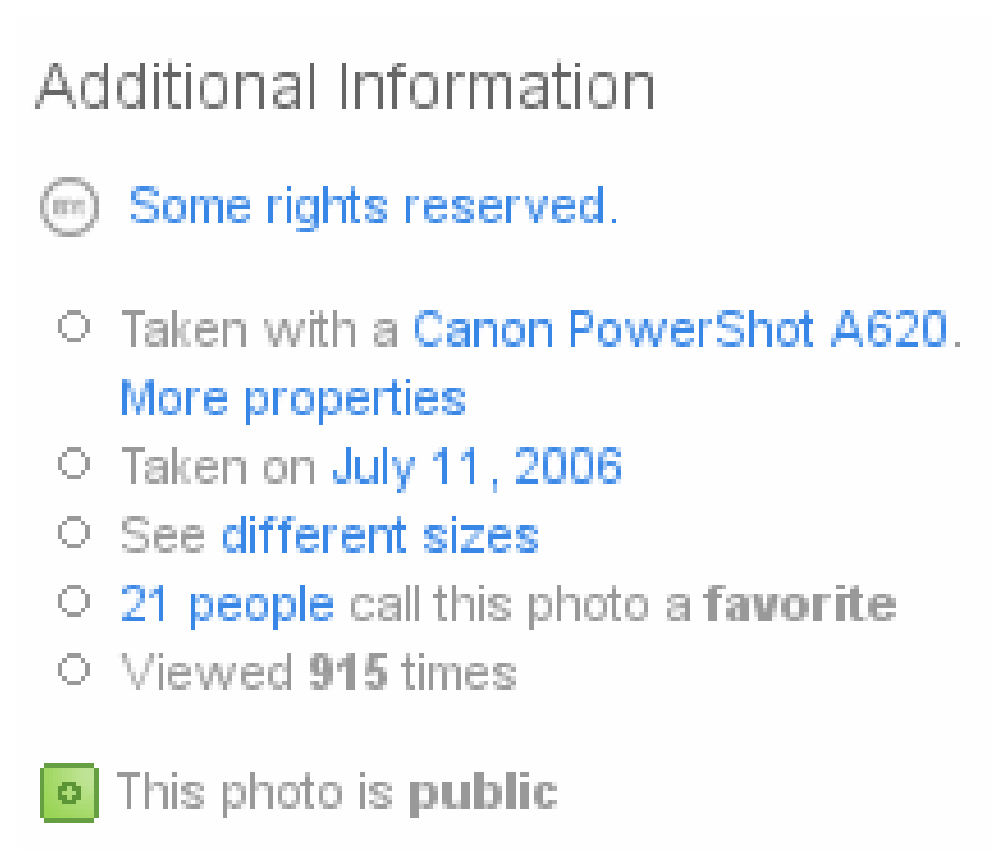
\includegraphics[width=0.9\marginparwidth]{scrsh_flickr_photo_metadata}
}

Flickr is a photo sharing site which are known to be on the cutting edge when
it comes to enabling new and innovating features in it's domain. Flickr has a
quite peculiar history as it started out as a massively multi player online
game. An environment for photo sharing within the game was added in 2004 which
quickly became more popular than the game itself. The focus of the company was
shifted and their new photo sharing community was bought by Yahoo! Inc. in
March 2005 \citep[p.~257]{livingston07}.

This subsequent
analysis of Flickr will be carried out as a registered user. One has to be
registered for interacting with the site in such a way that one leaves
persistent traces. The site has a open nature enabling anonymous access
to the majority of content.

\subsection{Thumbnails}

Already on the welcome page (\figureref{scrsh.flickr.welcome})
we're finding navigation links that are social of
nature. Four thumbnails functions as sample of the most recently uploaded
photos by other members of the community. One can either navigate straight to
a detailed page for each particular photo by clicking on the respective
thumbnail (Id 6, p.~\pageref{table:flickr.content.inventory.6})
or the profile of the uploader by clicking on their user
name (Id 7, p.~\pageref{table:flickr.content.inventory.7}). Such thumbnails
with minimal meta data (the uploader) are prevalent all over Flickr. Of the
120 pages we collected in our content inventory 26 of them contained
thumbnails. Most of these thumbnails
are giving users incentives to navigate using social means%
\sidenote[-4\onelineskip]{
  Apart from the few pages that only show a
  stream of your own thumbnails when you're browsing your
  own photos by various methods.
}.
Which photos these thumbnails portray is dynamic. That is to say that other
users' actions\dash{}uploading a photo, tagging a photo, taking a photo with a
specific camera, collecting photos into sets, and adding photos to a certain
group\dash{}all determine the navigational choices you as a user is
presented with.

\subsection{Meta-data}

We arrive on a photo detail page as in
\figureref{scrsh.flickr.photo.detail}
if we utilize one of these thumbnails for navigation. In addition to comments
on the photo we find meta-data as in 
\figureref{scrsh.flickr.photo.detail.metadata}
Meta-data include the date the photo was taken, the manufacturer and the model
of the camera that was used which are all so called Exif%
\sidenote{Exchangeable Image File: a specification for image file format used
in digital cameras.}
data. Flickr utilize this data by enabling navigation based both on the
dates a picture was taken and by camera make and model. Say you're trying to
find a picture from your home town on a particularly beautiful summer day. By
using date of picture taking based navigation coupled with tags or
geographical data (which both will be discussed shortly) you're probably
increasing you chances of finding what you want. Camera make information could
be useful when looking at the quality of pictures taken with certain cameras
before purchasing one yourself.

\begin{figure}
  \captionstyle{\raggedright}
  \begin{whole}
    \begin{minipage}[t]{0.475\wholewidth}
      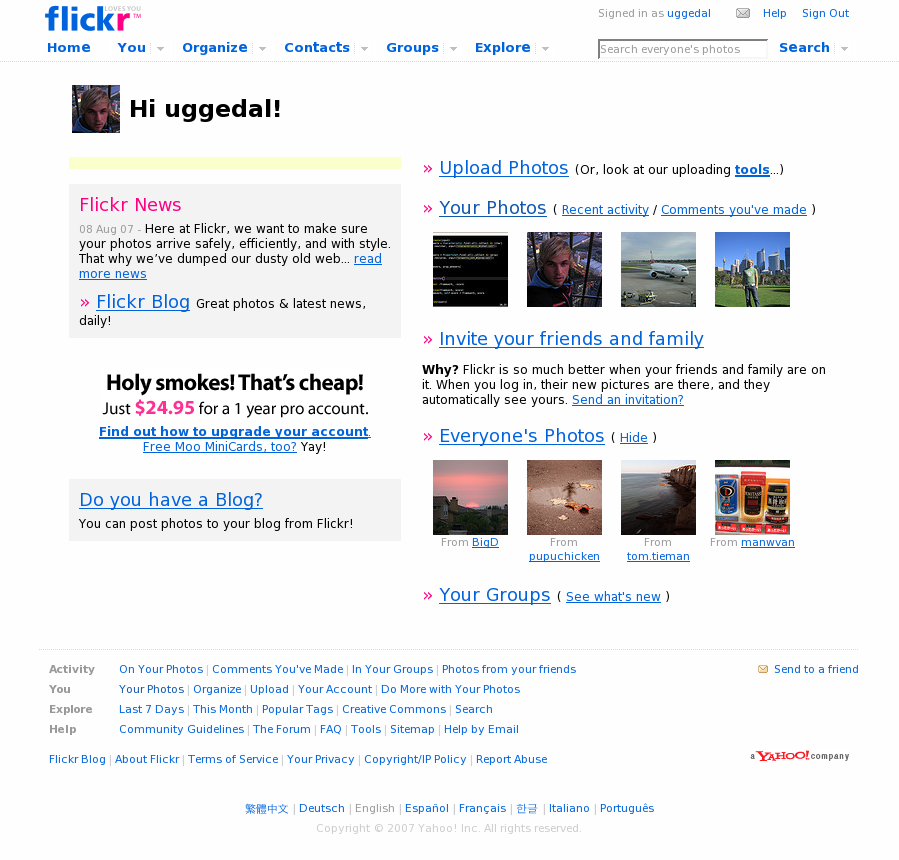
\includegraphics[width=\textwidth]{scrsh_flickr_welcome}
      \caption[Flickr Welcome Page]{%
         The Welcome Page,
         retrieved October 16, 2007, from \url{http://flickr.com}.}
      \label{figure:scrsh.flickr.welcome}
    \end{minipage}
    \hfill
    \begin{minipage}[t]{0.475\wholewidth}
      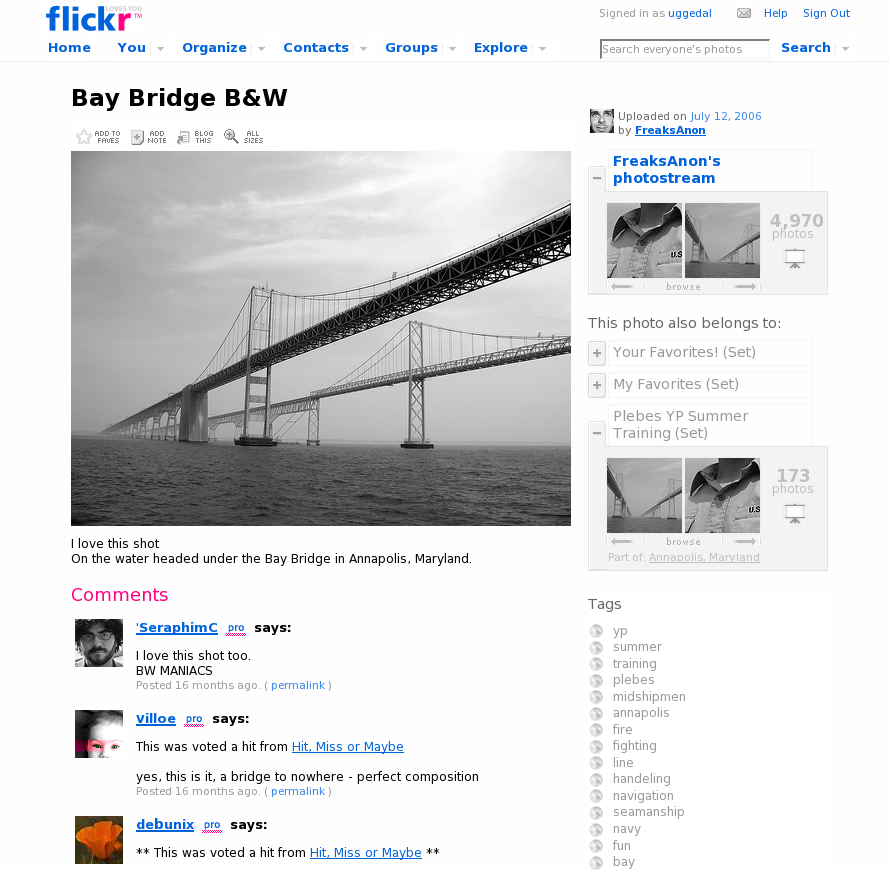
\includegraphics[width=\textwidth]{scrsh_flickr_photo_detail}
      \caption[Flickr Photo Detail Page]{%
         A Photo Detail Page,
         retrieved October 26, 2007, from
         \url{http://flickr.com/photos/benbengraves/187609810}.}
      \label{figure:scrsh.flickr.photo.detail}
    \end{minipage}
  \end{whole}
  \normalcaption
\end{figure}

\subsection{Folksonomy}
Of most importance
for Flickr, and indeed what makes Flickr a folksonomy, is it's tagging
abilities. Caterina Fake, co-founder of Flickr, explains it's importance as
\postquote[p.~261]{livingston07}{%
  Tagging really revolutionized the way the product behaved}
All registered user can label anyone's photos by applying such short
descriptive tags. This collaborative process lay the ground work for other
user's ability to easily browse photos by topic.
\figureref{scrsh.flickr.tagcloud}
exemplifies how the user generated data trough tagging can be used as a
navigational aid. A so called \emph{tag cloud} is used to visualize the
popularity (and thereby importance) of the individual tags. The larger the
tag title, the more frequent the tag has been applied to photographs.

Tag clustering was released in the fall of 2005 \citep{butterfield05} as a way
to easier see the relationships between separate tags. For any given tag a
cluster of three related tags is generated and displayed to users when they
are browsing as seen in
\figureref{scrsh.flickr.photo.detail}.
Flickr algorithmically generates these listings based on what tags users tend
to use together for labeling a photo.

Tagging is a very flexible approach only hindered by users' imagination. In the
early days of Flickr there was no support for geographical data. Users soon
found a remedy for this by tagging photos with longitude and latitude. By
using the same technology we're using in our prototype application
(Greasemonkey) they were able to integrate Google Maps%
\sidenote{
  Available at \url{http://maps.google.com}
} in Flickr, enabling user's to place their photos on a map and automatically
generate geographical coordinate tags%
\sidenote{
  More info about the early days of \emph{geotagging} can be found on the
  remains of the Flickr Geotagging group, available at
  \url{flickr.com/groups/geotagging/}.
}.

\subsection{Geographical data}

In late August 2006 Flickr introduced geotagging abilities
\citep{butterfield06} by integrating mapping aspects from Yahoo! Maps%
\sidenote{
  Available at \url{http://maps.yahoo.com}.
}
Users could now place their photos on a
map to signify where they were captured.
% Finish description.
% Take screen shot.
% Write about the new places feature.
% Write and cite when proper geo data was incorporated.

\subsection{Interestingness}
% Cite collaborative filtering. Introduced in same blog post as clustering.

\begin{figure}
  \begin{whole}
    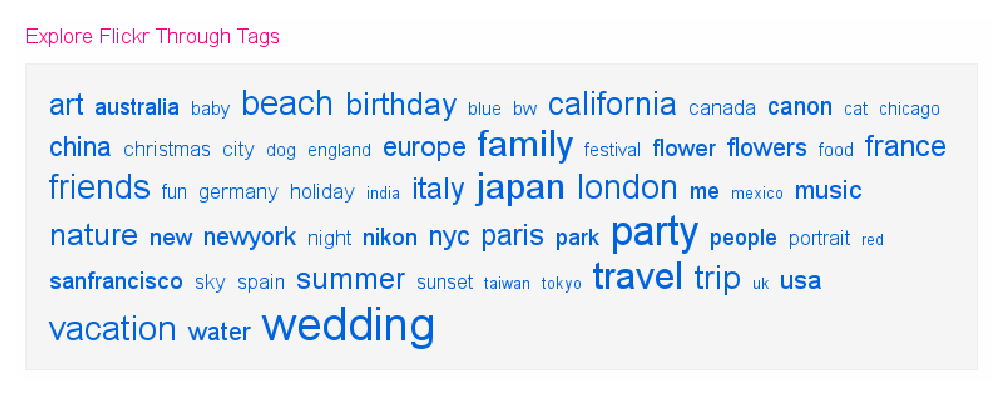
\includegraphics[width=\wholewidth]{scrsh_flickr_tagcloud}
    \caption[Flickr Tag Cloud]{%
       Tag Cloud,
       retrieved November 1, 2007, from \url{http://flickr.com/explore}.}
    \label{figure:scrsh.flickr.tagcloud}
  \end{whole}
\end{figure}

\begin{figure}
  \begin{whole}
    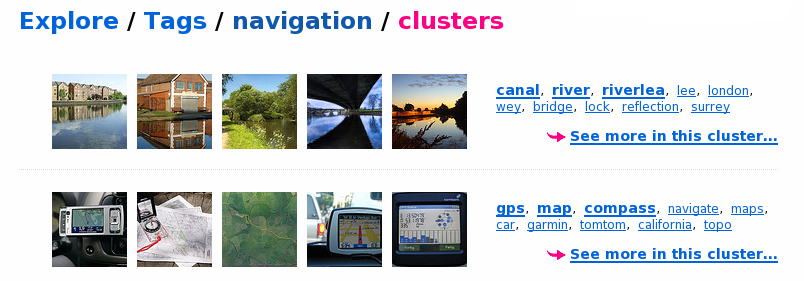
\includegraphics[width=\wholewidth]{scrsh_flickr_tagcluster}
    \caption[Flickr Tag Cluster]{%
       Tag Cluster,
       retrieved November 19, 2007, from
       \url{http://flickr.com/photos/tags/navigation/clusters/}.}
    \label{figure:scrsh.flickr.tagcluster}
  \end{whole}
\end{figure}

\section{Facebook}
\label{section:analysis.facebook}

\subsection{Profiles}

As we've seen pictures and their thumbnails and titles are central in Flickr.
In the same way user names and thumbnails of profile images are scattered all
trough Facebook. This is no mystery as the dominant entity of Facebook is
persons and their profile much as pictures' essentialness for Flickr.

\section{Amazon}

    \chapter{Selection of Third Party Software}
\label{chapter:selection.of.third.party.software}

Firstly one important aspect with the software stack used in our thesis work
\dash{}from operating system to third party libraries\dash{}is
that it should only consist of \term{open source}
\sidenote{
  Open source software was introduced as an alternative to
  \term{free software} in the hopes of avoiding confusion and making
  such software more  appropriate for the corporate world
  \citep[p.~7]{fogel05}.
  \work{The Open Source Definition} \citep{osind} dictates the terms
  software needs to follow to be accepted as open source.
}
software. In our experience it's
invaluable to have sources available for all involved software. If one
encounter abnormal behavior or bugs it's much easier to locate them when one
have sources available and one can trivially (depending on the complexity of
the problem) create a patch that sorts them out. One of the motivating factors
of open source contributors is the opportunity for other users to find and fix
failures and provide improvements on their code \citep[p.~87]{hippel05}.

It's also our experience that one can find third party software that fits
one's problem domain more easily if one chooses to use open source software
because of the vast availability of such software.
\citet{deshpande08} found that the availability of open source
code and projects had grown exponentially from January 1995 to December 2006.

Lastly it's of importance to keep the act of conducting science open so that
future researchers easily can discuss, falsify, and improve on previous
research. Software is often an essential part of computer science research and
\citet[p.~430]{kelty05} therefore argues that open source
is a property to strive for when conducting such research.

\section{Prototype Software Stack}

Based on the design decisions described in detail in
\chapterref{implementation}
we needed to figure out what parts
our software architecture should be composed of. 

\subsection{Client Side}

\subsubsection{Platform}
\label{section:implementation.architecture.client.side.platform}

The platform for the clients is in essence a web browser. We are making
changes to a web page after all. The web browser have to be explicitly chosen
to be one that readily supports scripting existing
web pages\dash{}a term often called \term{user scripting}.
The \project{Firefox}%
\sidenote{
  Available at \url{http://www.mozilla.com/en-US/firefox}.
}
web browser was the first browser providing a
plug-in for handling such scripting of web pages and seems to have the most
mature implementation in our view. Since Firefox also is the
most adopted%
\sidenote{
  According to \citet{onestat08} Firefox was the second most used web browser
  only surpassed by \project{Internet Explorer}.
}
cross-platform open source web browser the platform choice was quite easy.

Firefox provide user scripting trough the means of the
\project{Greasemonkey}%
\sidenote{
  Available at \url{http://greasespot.net}.
}
browser extension. Essentially all it provides is the ability for a user to
install a script which can manipulate the behaviour and properties of an
existing web page using the \term{\abbr{DOM}}%
\sidenote{
  The \abbr{DOM} is a three of objects representing the hierarchical
  structure of nested tags (with text and attributes) in \abbr{HTML}
  documents \citep[pp.~307--310]{flanagan06}.
}.
When a user have such a script for a specific web page installed it's
instructions will be executed on the next visit to the given site, enabling
all kinds of modifications to the \abbr{DOM}. Although most often used
for customizing the apperance of a given web site \citep[p.~39]{vitali06},
Greasemonkey can also be used for creating new navigational designs on the
\urort{} web site. Some have predicted that Greasemonkey 

Although we've settled on the Firefox and Greasemonkey platform there is a
certain possibility that our implementation could work in other browsers
providing user scripting. The \project{Opera} browser provides user scripting
without any plugins%
\sidenote{
  For more information see
  \url{http://www.opera.com/support/tutorials/userjs/examples}.
},
the \project{Safari} browser can handle user script with the
\project{GreaseKit}%
\sidenote{
  Available at \url{http://8-p.info/greasekit}.
}
plug-in. We have not tested such support for ourselves since we decided to
focus all our efforts on one platform and thereby not be subjected to
cross-browser diffrences\dash{}both in potential bugs and programmatic
interfaces.

\subsubsection{Programming Language}

The ability to programmatically alter behavior inside web browsers was first
introduced by \project{Netscape} in their 2.0 version of the web browser
with the same name. \project{JavaScript} was first intended to be a
lightweight scripting language for gluing together \abbr{HTML} and applets
written in the \project{Java} programming language \citep{netscape95}.%
\sidenote{
  Sun Microsystems, the creators of Java, had negotiated with
  Netscape about including it in their second major web browser release.
  The development of JavaScript, then called Mocha, was already
  underway and people inside Netscape wondered why one needed two
  languages.
  \postquote{eich08}{%
    The answer was that two languages were required to serve the two
    mostly-disjoint audiences in the programming ziggurat who most deserved
    dedicated programming languages: the component authors, who wrote in C++
    or (we hoped) Java; and the `scripters', amateur or pro, who would write
    code directly embedded in HTML}
}
Java applets never took off and JavaScript soon became the \latin{de facto}
standard for enabling behavior on the Web and was standardized as
\project{ECMAScript} in 1997 \citep{ecma99}.

Because of this we had no say in what programming language to use on the
client side. That is not to say that JavaScript is a poor programming
language. Contradictory to it's name, JavaScript bears few similarities to the
Java language.%
\sidenote{
  The name was more of a marketing decision when Netscape teamed up
  with Sun
  \citep[p.~2]{flanagan06}.
}
Despite it's origins as a scripting language JavaScript is now considered
a full-featured modern programming language
\citedouble{p.~2}{flanagan06}{p.~3}{resig06}.

\subsubsection{Convenience Library}

We decided to use a JavaScript library to make interactions with the
\abbr{DOM} simpler.
In addition there recent JavaScript convenience libraries provide a
unified interface to the browser\dash{}abstracting away inconsistencies
between browser vendors. Lately a myriad of such frameworks have appeared,
but the most interesting ones seems to be
\project{Prototype},
\project{Yahoo! UI Library} (\abbr{YUI} for short),
\project{MooTools},
\project{MochiKit}, and
\project{jQuery}.%
\sidenote{
  Available, in respective order, at
  \url{http://www.prototypejs.org},
  \url{http://developer.yahoo.com/yui},
  \url{http://mootools.net},
  \url{http://mochikit.com}, and
  \url{http://jquery.com}.
}
There are other frameworks available that provide everything but the kitchen
sink but we needed a lightweight or modular solution.

As can be seen in the following table we summarized the size of the most
current version for each library of this writing. These are not exact
metrics\dash{}we selected not to include certain widgets and logging
facilities for the modularized libraries\dash{}but should provide clear
guidance. To keep a level playing feel in this comparison we did not use
minified (removal of comments and unnecessary spaces) or packaged (compressed)
versions of the libraries. All comments and documentation was stripped with a
small script presented in \sourcecodepageref{javascript.comment.sripping}
since the in-line documentation and commenting varied amongst the libraries.

\sidetable{JavaScript Library Comparison
           \label{table:javascript.library.comparision}}{%
  
  \begin{tabular}{lr}

    Library & Size \\
            & (kB) \\
    \midrule

    MooTools (1.11)     & 67 \\
    jQuery (1.2.3)      & 91 \\
    Prototype (1.6.0.2) & 122 \\
    MochiKit (1.3.1)    & 181 \\
    \abbr{YUI} (2.5.0)  & 286 \\

  \end{tabular}
}

We played around a bit with the different libraries to get a feel for how
they worked. What follows is a comparison of simple \abbr{DOM} manipulation
for the different libraries. We followed the official documentation for the
various libraries and tried to solve or problem as succinct and clearly as
possible. We tried to add a \code{class} attribute of \val{highlight} to
all \code{em} elements with an descendant \code{p} element: 

\begin{scode}{Java}{dom.manipulation.prototype}{%
  \abbr{DOM} Manipulation with Prototype}{%
  DOM manipulation in JavaScript with the Prototype library}
\begin{lstlisting}
getElementsBySelector("p em").each(function(em) {
  em.addClassName("highlight");
});
\end{lstlisting}
\end{scode}

\begin{scode}{Java}{dom.manipulation.yui}{%
  \abbr{DOM} Manipulation with Yahoo! \abbr{UI} Library}{%
  DOM manipulation in JavaScript with the Yahoo! UI library}
\begin{lstlisting}
var em = YAHOO.util.Selector.query("p em"); 
YAHOO.util.Dom.setClass(em, "highlight);
\end{lstlisting}
\end{scode}

\begin{scode}{Java}{dom.manipulation.mootools}{%
  \abbr{DOM} Manipulation with MooTools}{%
  DOM manipulation in JavaScript with the MooTools library}
\begin{lstlisting}
$$("p em").each(function(em){
  em.addClass("highlight");
});
\end{lstlisting}
\end{scode}

\begin{scode}{Java}{dom.manipulation.mochikit}{%
  \abbr{DOM} Manipulation with MochiKit}{%
  DOM manipulation in JavaScript with the MochiKit library}
\begin{lstlisting}
var p = getElementsByTagAndClassName("p");
for (i = 0; i < p.length; i++) {
  em = getElementsByTagAndClassName("em","*", p[i]);
  for (j = 0; j < em.length; j++) {
    addElementClass(em, "highlight");
  }
}
\end{lstlisting}
\end{scode}

\begin{scode}{Java}{dom.manipulation.jquery}{%
  \abbr{DOM} Manipulation with jQuery}{%
  DOM manipulation in JavaScript with the jQuery library}
\begin{lstlisting}
$("p em").addClass("highlight");
\end{lstlisting}
\end{scode}

When we compare these rather trivial problem solutions it becomes apparent
that choosing a JavaScript library can have major impact on how easily
implemented and understood your code will be. Four of the five libraries
have support for selector syntax based on
that found in\abbr{CSS}%
\sidenote{
  Cascading Style Sheets. A stylesheet language for describing the
  presentation of for instance \abbr{HTML} documents.
}.
This is what makes the MochiKit example the most complex one, requiring the
developer to do two queries into the \abbr{DOM} and construct two
loop structures for iterating over the results.
Prototype and MooTools also requires the developer to loop over a single
result set, but the iteration is abstracted into an \code{each} function
making the logic a bit more clearer. Yahoo! \abbr{UI} Library's \abbr{DOM}
functions works on both single elements and collections of
elements\dash{}eliminating the need for an explicit loop structure.
Notice though that the library from
Yahoo! relies heavily on namespacing\dash{}which is a good thing for
interoperability with other libraries\dash{}but can be a bit verbose at times.

The solution written with jQuery provides even more clarity.
Every query into the \abbr{DOM} returns a special jQuery object which means
that one can call methods like \code{addClass} directly on this object
regardless if the jQuery object holds a single or multiple elements.
Also unique to jQuery is the fact that every method call returns a new jQuery
object. This means that one can \term{chain} methods together, expressing
succinctly and clearly what you intend to accomplish with your code. We can
extend our initial problem and add some punctuation inside our \code{em}
element:

\begin{scode}{Java}{jquery.method.chaining}{%
  jQuery Method Chaining}{%
  Chaining multiple methods together in jQuery}
\begin{lstlisting}
$("p em").addClass("highlight").append("!");
\end{lstlisting}
\end{scode}

Based on the minimal file size jQuery provided (only outbested by MooTools)
and it's clear and unique syntax we decided on selecting it as the JavaScript
library for our implementation. It seems others have take jQuery and it's
virtues to hart as many large corporations like Google, Intel, Dell, and
\abbr{BBC} have used it in their public facing offerings.%
\sidenote{
  For a complete list see \url{http://docs.jquery.com/Sites_Using_jQuery}.
}

\subsection{Server Side}

\subsubsection{Platform}

\subsubsection{Programming Language}

When doing prototype work it's important that the programming language one
uses is efficient to work with. This means that programmer efficiency is more
important than computational efficiency (a language's native performance).
Since we didn't have time to invest in learning a new language we had to do
with those we knew from before. Of those \project{Ruby}%
\sidenote{
  Ruby recedes at \url{http://ruby-lang.org}.
},
\project{Python}%
\sidenote{
  The home of Python is \url{http://python.org}.
}, and
\project{Common Lisp}%
\sidenote{
  Common Lisp, the prevalent Lisp dialect today, is a standard \citep{ansi96}
  and has many implementations.
  A gateway to this language and it's many implementations can be found
  at \url{http://common-lisp.net}.
}
were the ones with language features that fitted our development process.

They are all \term{latent typed}%
\sidenote{
  Latent typing ``is a style of typing that does not require (or perhaps even
  offer) explicit type declarations''\citep{wikipedia08latent}.
}
and have quite expressive syntax. This makes for concise source code.
\citet{yegge07} argues that the worst thing that can happens to a code base is
size which often is the result of code bloat. In addition, both Ruby, Python,
and Common Lisp are \term{interpreted} languages%
\sidenote{
  This is only partly true since Common Lisp implementations incrementally
  compile code and extensions or new implementations for Python and Ruby
  implements just-in-time compilers. In both cases the developer
  does not need to explicitly invoke a compile process before using
  a program, therefore resembling interpreted languages.
}.
This means that the programmer don't have to go trough a compilation process
before he can see the results of his labor. When prototyping rapidly it's
quite convenient to make small changes and see the results instantanously.

Disussion of the virtues of different flavors and implementations of
programming languages have been the subject of endless debate.
In the end we think it comes down to
personal preference and making a pragmatic choice for the tool best suited for
the job at hand. If we had to select a programming language based on our list
of candidates based on the languages syntax and posibilities in itself we
would probably have gone with Common Lisp. \citet[p.~27]{foderaro91} have
called it ``the programmable programming language''based on the fact that
program code in Lisp is data and can be manipulated with the same constructs
one are using on data. This makes it immensly powerfull and is the reason why
it's survived for over 50 years \citep[p.~217]{mccarthy78}
and been able to adopt new paradigms in programming as they've appered.
Even though we walue programming efficiency over computational performance,
it should be noted that Common Lisp have been described as the only performant
dynamic language \citep{martin08} compared to statically compiled languages%
\sidenote{
  In \work{The Computer Language Benchmarks Game} several programming
  languages are pitched against each other in several tests to determine
  their computational performance. As of this writing (April 2, 2008)
  Common Lisp is 1.8 times slower than the fastest language: C++. Python
  and Ruby are respectively 18 and 56 times slower than the leader.
  Updated results can be found at
  \url{http://shootout.alioth.debian.org/gp4/benchmark.php?test=all&lang=all}.
}.

As it turns out, the most important criteria for choosing our implementation
language was it's library support. In the next section we discuss our options
of such libraries or frameworks. Based on our findings there we landed on
Ruby as the language of our server side implementation.

\subsubsection{Data Extraction Library}

The core library we need is one that handles data extraction from existing
web pages, so called \abbr{HTML} \term{scraping}. While it's possible to
handle such problems with regular expressions, this becomes tedious after a
while. We therefore prefer a special purpose library.

The major deciding factor when we selected the implementation language was
the availability of such a library and it's usefulness. We've already
revealed Ruby as our implementation language and are therefore killing the
suspense. Our data extraction library of choice is called \project{Hpricot}%
\sidenote{
  Hpricot can be obtained from \url{http://code.whytheluckystiff.net/hpricot}.
  A curious note: Hpricot is written by the same person who created
  Hoodwink.d\dash{}our inspiration for a transparent prototype implementation.
}
and makes \abbr{HTML} parsing a blissful endeavor in our opinion.

The Python alternative for web page scraping is \project{Beautiful Soup}.
We were not able to find any libraries specially made for \abbr{HTML} scraping
implemented in Common Lisp. There exists several \term{\abbr{XML}}%
\sidenote{
  Extensible Markup Language. General purpose markup language specification
  that enables implementors to create custom markup languages.
  \abbr{HTML} is not a subset (specified in) \abbr{XML} \citep{w3c99}.
  \term{\abbr{XHTML}} on the other hand, a reformulated version of
  \abbr{HTML}, is a subset of \abbr{XML} \citep{w3c02}.
}
libraries that could handle our tasks, but none as well integrated as
the Ruby and Python options.

To get a feel for the difference between Hpricot and Beautiful Soup we tried
them out on some trivial examples. Under you'll see the listings for one
of these examples. We are trying to find an \code{em} element with a class
of \code{citation}, which have a \code{p} element as it's parent,
in a \abbr{HTML} document contained in the \code{html} object:

\begin{scode}{Python}{parsing.beautiful.soup}{%
  Parsing with Beautiful Soup}{%
  HTML parsing in Python with Beautiful Soup}
\begin{lstlisting}
html('p').content.findNextSiblings('em', 'citation')
\end{lstlisting}
\end{scode}

\begin{scode}{Ruby}{parsing.hpricot}{%
  Parsing with Hpricot}{%
  HTML parsing in Ruby with Hpricot}
\begin{lstlisting}
  html/'p > em.someclass'
\end{lstlisting}
\end{scode}

We feel that Hpricot's syntax is much clearer than that of Beautiful Soup.
This could be a personal preference since we've used \abbr{CSS} for a long
time and Hpricot's selector syntax is based on \abbr{CSS} and Xpath, just as
jQuery. Hpricot was in fact initially based on jQuery's selector syntax
\citep{why06}. This means that we can use the same syntax for selectors on the
server and client side\emph{}a cognitive advantage.

\subsubsection{Data Fetching Library}

Since we've selected Ruby as our development language of choice we used
\executable{open-uri}, part of the standard Ruby library, for fetching
documents over \abbr{HTTP}%
\sidenote{
  Hyper Text Transfer Protocol. The data transfer protocol for the Web.
}.
\executable{open-uri} is trvial to use and integrates nicely with Hpricot:

\begin{scode}{Ruby}{fetching.openuri.parsing.hpricot}{%
  Fetching and Parsing with Hpricot and open-uri}{%
  Fetching a HTML document with \executable{open-uri}
  and parsing it with Hpricot to find the first and
  last name of a hCard Microformat}
\begin{lstlisting}
require 'hpricot'
require 'open-uri'

html = Hpricot(open('http://redflavor.com'))
(html/'address.vcard > .fn').inner_html
# => "Eivind Uggedal"
\end{lstlisting}
\end{scode}


\subsubsection{\abbr{JSON} Web Framework}

A web framework or rather \abbr{HTTP}
framework is needed to make the
collected data available for our client. Since we'll only be serving requests
for our JavaScript based client implementation we found it sound to transfer
this data as \abbr{JSON}%
\sidenote{
  \abbr{JSON}, short for JavaScript Object Notation, is specified in
  \abbr{RFC} 4627 \citep{crockford06}. Shortly put it's a lightweigh data
  interchange format based on the object literals of JavaScript.
}.
Luckily for us there exists a framework for Ruby for handeling such tasks
called \project{Halcyon}%
\sidenote{
  Halcyon can be found at \url{halcyon.rubyforge.org}.
}.
This framework makes the process of developing a web application for serving
\abbr{JSON} requests quite easy. It builds on \project{Rack}%
\sidenote{
  Rack is available at \url{rack.rubyforge.org}.
},
a web server interface that sits between a web framework and a web server. By
using Rack we can easily swap between different web servers that support the
protocoll mandated by Rack's interface layer. To demonstate the simplicity of
this framework we'll show how a simple greeting application could be
implemented:

\begin{scode}{Ruby}{halcyon}{%
  Hello World with Halcyon}{%
  A simple hello world application with Halcyon}
\begin{lstlisting}
class Hello < Halcyon::Server::Base
  route {|r| r.match('/').to(:action => 'greet') }
  
  def greet
    msg = {:interjection => 'hello',
           :noun         => 'world',
           :suffix       => '!'}
    ok(msg)
  end
end
\end{lstlisting}
\end{scode}

What is interesting is that the Ruby \code{msg} key/value hash is serialized
automitically to \abbr{JSON} when a client requests this resource:

\begin{scode}{Java}{halcyon.result}{%
  Client Result with Halcyon}{%
  The result of a client request to the Halcyon hello world application}
\begin{lstlisting}
{"status": 200,
 "body": {"interjection": "hello",
          "noun":         "world",
          "suffix":       "!"}}
\end{lstlisting}
\end{scode}

\subsubsection{Web Server}

Since our web framework builds on Rack we have several web servers to select
from.

% which webserver we selected, and why (mongrel, thin)
% prototype application. load balancing not that important with
% for instance nginx.


\subsubsection{Persistance Library}

We decided to use an \abbr{ORM}%
\sidenote{
  % define
}
for abstracting our persistance handeling. With such a solution we could
change relational database engines transparently if  neccesary. In addition
\abbr{ORM} libraries often provide a nice interface to the database
eliminating the need for constructing complex \abbr{SQL}%
\sidenote{
  % define
}. The most popular \abbr{ORM} libraries for the Ruby language are%
\sidenote{
  Available at respectively
  \url{http://rubyforge.org/projects/activerecord},
  \url{http://datamapper.org}, and
  \url{http://sequel.rubyforge.org}.
}:

\begin{items}
  \iterm{ActiveRecord} %describe
  \iterm{DataMapper} % describe
  \iterm{Sequel} %describe
\end{items}


\section{Development Tools}

As with the implementation platforms, languages, and third party libraries
our first criterion for selecting development tools is freedom.

\subsection{Version Control}

We've found it indispensable to use \term{version control} when writing code
and even used it when authoring this thesis. We'll not spend time to discuss
the merits of version control since we feel it's benefits are major and
using one induces almost zero overhead in your working process. Sometimes we
feel that the use of version control can guide you when conducting complex
tasks.

There are however several different forms of version control system one can
use. One of the most used version control implementations the last years
in open source circles was
\project{Subversion}%
\sidenote{
  Available at \url{http://subversion.tigris.org}.
}\dash{}a \term{centralized version control system} meaning that one central
server holds the version controlled code repository and it's history.%
\sidenote{
  Developers on the client side have working copies and need to contact the
  centralized server to get a hold of historical data and create new history.
}
Recently \term{decentralized version control systems} have become more popular
amongst developers. A decentralized model means that every developer can have
their own repository consisting of all history.%
\sidenote{
  You can for instance be without internet connectivity and still commit
  changes, revert to previous versions, and handle all other tasks your
  version control system supports.
}
Code is then shared either in a push or pull fashion between such individual
repositories. This enables a much better model for collaboration.
We favor this last model of version control and so have projects
like \project{Linux}, \project{X}, \project{Mozilla},
and \project{OpenSolaris}.%
\sidenote{
  \citeauthor{torvalds07}, author of the Linux kernel,
  have described Subversion and centralized version control
  as fundamentally flawed since it's supposed to be a
  \q{\abbr{CVS} done right}. Since he feels \abbr{CVS} is flawed Subversion
  is therefore inherently flawed \citeyearpar{torvalds07}.
}

Based on criteria of performance and current adoption there are in our view
only two interesting decentralized version control systems:
\project{Git}%
\sidenote{
  Available at \url{http://git.or.cz}.
}
and \project{Mercurial}%
\sidenote{
  Available at \url{http://www.selenic.com/mercurial}.
}. Both are unique in that they don't track meta-data, they just track
content and meta-data are thereby inferred from the content.
At a very high level view Mercurial have a better user interface and Git
supports some advanced features the former don't have. We opted to used
Mercurial for this development project since we've substantial experience in
using it and did not need any of Git's advanced features.

\subsection{Editor}

A developer's main tool for authoring software is his editor. Sometimes the
language of implementation warrants a specialized editor with aids for
handling cumbersome tasks specific to that language. Such an editor is often
called an \abbr{IDE}%
\sidenote{
  A good example of an \abbr{IDE} (integrated development environment
  for short) is \project{Eclipse} (available at \url{http://eclipse.org}).
  It was first used for Java development but since extended with
  plugins for handling other programming languages and families.
}
and are used most often for languages like Java and C\#.
\citet{murphy06} found that developers mostly use an \abbr{IDE} for navigating
large collections of source code, refactoring code, debugging code, and
interacting with revision control systems in addition to normal editor usage.
Development environments found in Lisp%
\sidenote{
  \prequote[p.~69]{sandewall78}{%
    describes the nature and benefits of the Lisp environment as}{%
      The `residential' design of programing systems, whereby all facilities
      for the user are integrated into one system with which the user
      communicates during the entire interactive session, offers great
      possibilities for user convenience}
}
and Smalltalk%
\sidenote{
  Similar to Lisp's programming environment
  \postquote[p.viii]{goldberg83}{%
    Smalltalk is designed so that every component in the system that is
    accessible to the user can be presented in a meaningful way for
    observation and manipulation}

}
are surpassing \abbr{IDE} types in integration and interactiveness even though
they preceded them.

The programming languages we previously settled on, JavaScript and Ruby,
are very expressive and dynamic in their nature in addition to being
interpreted instead of compiled. Our experience is that \abbr{IDE} usage for
such languages stands more in the way than aid you as a programmer during
your problem solving process.
\citet{bray07} conducted a rather unscientific survey of 1000 Ruby
programmers. Despite of the surveys shortcomings it showed that
the majority of Ruby programmers used non-\abbr{IDE} editors for their
development.

The interactive experience provided by Lisp and Smalltalk implementations are
sadly missing%
\sidenote{
  Ruby has an interactive interpreter similar to those found in Lisp and
  Smalltalk environments called \executable{irb}. It's not integrated into an
  overall programming environment and therefore is mostly used for testing out
  small ideas.
}
from JavaScript and Ruby implementations. This means that we're left with
finding a good editor which enables us to focus on writing code as efficiently
and safely as possible. Editor selection is highly a matter of preference and
finding one that matches your work process. Powerful editors have a
reputation of being quite hard to learn. But if you get over the steep
learning curve the benefits the editor gives you are worth it.
\citeauthor{orenstein08} have experienced how much effort programmers can
invest in something seemingly trivial as an editor:

\begin{citequote}{orenstein08}
  If the thought of switching editors doesn't fill you with quite a bit of
  dread, what you're using now is almost certainly under powered, and you
  definitely haven't customized it enough.
\end{citequote}

    \chapter{Implementation}
\label{chapter:implementation}

% This chapter should include design choices for my implementation. For
% example choices taken for generating relevant data for test users
% and a computational sound method for doing so. As JavaScript in browsers are
% quite inefficient it will probably be necessary to persist data at a server
% in some sort of cache. The clients could then get this data by invoking a
% single request. The result could for instance be JSON serialized. Scraping
% of such data is probably done more efficient and safer at the server side
% since multiple XMLHttpRequests in the clients for scraping and parsing could
% prove to be quite computational expensive.

As we've seen in 
\sectionref{building.on.top.of.the.web}
it's possible to build applications on top of existing web sites by creating
transparent prototype implementations. This chapter starts with an account of
what kind of navigation system we wanted to build, goes on to describe why we
decided on such navigational designs, and concludes with an explanation of how
the implementation was built\dash{}the ingredients of our implementation.

\section{Design}

\section{Process}
% Prototype, exploratory
% TDD, BDD

\section{Architecture}

Firstly one important aspect with the software stack used in this
implementation\dash{}from operating system to third party libraries\dash{}is
that it's only consisting of open source software.

We decided to use a server--client architecture so that we could move some of
the more computationally expensive operations off the client and into a
dedicated server. Another benefit of such an architecture is that it allows us
to cache data globally\dash{}shared by all clients.

\subsection{Client Side}

\subsubsection{Plattform}
\label{section:implementation.architecture.client.side.plattform}

The plattform for the clients is in essence a web browser. We are making
changes to a web page afteral. The web browser have to be explicitly choosen
to be one that readily supports scripting existing
web pages\dash{}a term often called \term{user scripting}.
The \project{Firefox}%
\sidenote{
  Available at \url{http://www.mozilla.com/en-US/firefox}.
}
web browser was the first browser providing a
plugin for handeling such scripting of web pages and seems to have the most
mature implementation in our view. Since Firefox also is the
most adopted%
\sidenote{
  According to \citet{onestat08} Firefox was the second most used web browser
  only surpassed by \project{Internet Explorer}.
}
cross-platform open source web browser the plattform choice was quite easy.

Firefox provide user scripting trough the means of the
\project{Greasemonkey}%
\sidenote{
  Available at \url{http://greasespot.net}.
}
browser extension. Essentially all it provides is the ability for a user to
install a script which can manipulate the contents of a web page
in various ways using the \abbr{DOM}%
\sidenote{
  % write from js book.
}.
When a user have such a script for a specific web page installed it's
instructions will be executed on the next visit to the given site, enabeling
all kind of modifications possible in the \abbr{DOM}.

Although we've setteled on the Firefox and Greasemonkey plattform there is a
certain possibility that our implementation could work in other browsers
providing user scripting. The \project{Opera} browser provides user scripting
without any plugins%
\sidenote{
  For more information see
  \url{http://www.opera.com/support/tutorials/userjs/examples}.
},
the \project{Safari} browser can handle user script with the
\project{GreaseKit}%
\sidenote{
  Available at \url{http://8-p.info/greasekit}.
}
plugin. We have not tested such support for ourselves since we decided to
focus all our efforts on one plattform.

\subsubsection{Programming Language}

Programming behaviour inside web browsers was first introduced by

Because of this we had no say in what programming language to use on the
client side. That is not to say that JavaScript is a poor programming
language.
% list it's good features, and that recently the style of js has changed. cite
% js pro book. cite js ref book.
% cite stewe yegge about next big lanuage

\subsubsection{Framework}

We decided to use a JavaScript library to make interactions with the DOM
simpler. Lately a myriad of such frameworks have appered, but the most
interesting ones seems to be
\project{Prototype},
\project{Yahoo! UI Library},
\project{MooTools},
\project{MochiKit}, and
\project{jQuery}.%
\sidenote{
  Available, in respective order, at
  \url{http://www.prototypejs.org},
  \url{http://developer.yahoo.com/yui},
  \url{http://mootools.net},
  \url{http://mochikit.com}, and
  \url{http://jquery.com}.
}
There are other frameworks available that provide everything but the kitchen
sink but we needed a lightweight solution.

% jQuery ++ for it's css (+xpath) based selectors
% jQuery ++ for it's size
% jQuery ++ for it's method chaining

\subsection{Server Side}

\subsubsection{Plattform}

\subsubsection{Programming Language}

\subsubsection{Framework}

\section{Development Tools}

As with the implementation plattforms, languages, and third party libraries
our first criterion for selecting development tools is freedom.

\subsection{Version Control}

We've found it indispensable to use \term{version control} when writing code
and even used it when authoring this thesis. We'll not spend time to discuss
the merrits of version control since we feel it's benefits are major and
using one induces almost zero overhead in your working process. Sometimes we
feel that the use of version control can guide you when conducting complex
tasks.

There are however several different forms of version control system one can
use. One of the most used version control implementations the last years
in open source cicles was
\project{Subversion}%
\sidenote{
  Available at \url{http://subversion.tigris.org}.
}\dash{}a \term{centralized version control system} meaning that one central
server holds the version controlled code repository and it's history.%
\sidenote{
  Developers on the client side have working copies and need to contact the
  centralized server to get a hold of historical data and create new history.
}
Recently \term{decentralized version control systems} have become more popular
amongst developers. A decentralized model means that every developer can have
their own repository consisting of all history.%
\sidenote{
  You can for instance be without internet connectivity and still commit
  changes, revert to previous versions, and handle all other tasks your
  version control system supports.
}
Code is then shared either in a push or pull fashion between such individual
repositories. This enables a much better model for collaboration.
We favor this last model of version control and so have projects
like \project{Linux}, \project{X}, \project{Mozilla},
and \project{OpenSolaris}.%
\sidenote{
  \citeauthor{torvalds07}, author of the Linux kernel,
  have described Subversion and centralized version control
  as fundamentally flawed since it's supposed to be a
  \q{\project{CVS} done right}. Since he feels CVS is flawed Subversion
  is therefore inherently flawed \citeyearpar{torvalds07}.
}

Based on criteria of performance and current adoption there are in our view
only two interesting decentralized version control systems:
\project{Git}%
\sidenote{
  Available at \url{http://git.or.cz}.
}
and \project{Mercurial}%
\sidenote{
  Available at \url{http://www.selenic.com/mercurial}.
}. Both are unique in that they don't track meta-data, they just track
content and meta-data are thereby infered from the content.
At a very high level view Mercuial have a better user interface and Git
supports some advanced features the former don't have. We opted to used
Mercurial for this development project since we've substantial experience in
using it and did not need any of Git's advanced features.

\subsection{Editor}

A developer's main tool for authoring software is his editor. Sometimes the
language of implementation warrants a specialized editor with aids for
handeling cumbersome tasks specific to that language. Such an editor is often
called an \abbr{IDE}%
\sidenote{
  A good example of an \abbr{IDE} (integrated development environment
  for short) is \project{Eclipse} (available at \url{http://eclipse.org}).
  It was first used for Java development but since extended with
  plugins for handeling other programming languages and families.
}
and are used most often for languages like Java and C\#.
\citet{murphy06} found that developers mostly use an \abbr{IDE} for navigating
large collections of source code, refactoring code, debugging code, and
interacting with revision control systems in addition to normal editor usage.
Development environments found in Lisp%
\sidenote{
  \prequote[p.~69]{sandewall78}{%
    describes the nature and benefits of the Lisp environment as}{%
      The `residential' design of programing systems, whereby all facilities
      for the user are integrated into one system with which the user
      communicates during the entire interactive session, offers great
      possibilities for user convenience}
}
and Smalltalk%
\sidenote{
  Similar to Lisp's programming environment
  \postquote[p.viii]{goldberg83}{%
    Smalltalk is designed so that every component in the system that is
    accessible to the user can be presented in a meaningful way for
    observation and manipulation}

}
are surpassing \abbr{IDE} types in integration and interactivness even though
they preceded them.

The programming languages we previously settled on, JavaScript and Ruby,
are very expressive and dynamic in their nature in addition to beeing
interpreted instead of compiled. Our experience is that \abbr{IDE} usage for
such languages stands more in the way than aid you as a programmer during
your problem solving process.
\citet{bray07} conducted a rather unscientific survey of 1000 Ruby
programmers. Despite of the surveys shortcommings it showed that
the majority of Ruby programmers used non-\abbr{IDE} editors for their
development.

The interactive experience provided by Lisp and Smalltalk implementations are
sadly missing%
\sidenote{
  Ruby has an interactive interpreter similar to those found in Lisp and
  Smalltalk environments called \executable{irb}. It's not integrated into an
  overall programming environment and therefore is mostly used for testing out
  small ideas.
}
from JavaScript and Ruby implementations. This means that we're left with
finding a good editor which enables us to focus on writing code as efficiently
and safely as possible. Editor selection is highly a matter of preference and
finding one that matches your work process. Powerfull editors have a
reputation of beeing quite hard to learn. But if you get over the steap
learning curve the benefits the editor gives you are worth it.
\citeauthor{orenstein08} have experienced how much effort programmers can
invest in something seemingly trivial as an editor:

\begin{citequote}{orenstein08}
  If the thought of switching editors doesn't fill you with quite a bit of
  dread, what you're using now is almost certainly underpowered, and you
  definitely haven't customized it enough.
\end{citequote}



    \chapter{Discussion}
\label{chapter:discussion}

This chaper will include a syntesis based on the analysis of our collected
data. The larger lines of our findings will be presented and we'll try to
represent a new and refreshed terminology for the field of social navigation
by the means of a taxonomy including patterns of navigational use.

    \chapter{Conclusion}
\label{chapter:conclusion}

The results of the research which we have provided in this thesis can be
categorized into three venues:

\begin{enum}
  \item We have given a structured overview of the field of social navigation
    as seen both in academic literature and in some noticeable social web
    sites.
  \item We have provided details of how one can implement unobtrusive
    prototypes in established spaces and the feasibility of such a technical
    approach.
  \item We have contributed knowledge of how activity streams functions as
    a social navigation technique on the \urort{} web site.
\end{enum}

Based on these three venues we'll provide the most important lessons to take
away from our research before we discuss possible future work in these fields.

\section{Lessons Learnt}

We believe there are both some theoretical and practical lessons to take away
from our research

\subsection{Social navigation}

As viewed in academic literature social navigation can mean different things.
We proposed a new definition of social navigation based on our belief in the
importance of peers in a social navigation system.%
\sidenote{
  The definition can be found in
  \sectionref{flickr.facebook.discussion.peers}.
}
This means that the information given from other people which guide navigation
have to come from peers within the system where navigation are conducted to be
considered social navigation.

Information given by the creators or 
editors of a web site are therefore not social navigation when used for
navigational purposes.
The creators can however implement structures in their web pages where users
of the system can impose information which can be used for social navigation.
One example of this divide can be found in recommender systems. Content based
recommendations is not social navigation since the information used
in the navigational process are given by the editors of the web page.
Recommendations given by collaborative filtering is on the other hand social
navigation since the navigational information is given by peers in the system.

\subsection{Unobtrusive prototyping}

Creating unobtrusive prototypes with Greasemonkey have its advantages and
disadvantages when used in real world experiments.

Greasemonkey is best fitted for situations where you don't have access to the
established web site one are prototyping on. If one have access to the inner
workings of a web site, it would probably be more efficient and easier to
implement the prototype within the established implementation. Another benefit
of modifying the web site implementation itself is the elimination of the
Greasemonkey and user-script installation process in addition to wider browser
support.

We found the major disadvantage of using Greasemonkey in a real world
experimental setting to be this complicated installation process and limited
browser support. We contribute this as the major factors for the high
non-accomplish rates we witnessed. Having conducted experiments in a
laboratory setting where users used pre-configured machines would have
mediated this problem.

\subsection{Activity streams}

Based on our experiment with activity streams on \urort{} we have provided
inconclusive findings of the success of such a social navigation technique.
We take our results as indications of the usefulness of activity streams.
Further research is needed to abandon the idea or recommend its usage.
Since we did not find any noticeable negative results towards activity streams
we can recommend implementations or prototypes of this feature in web sites
with similar dynamics as \urort{}.

\section{Future Work}

Our new definition of social navigation in light of the essentialness of peers
were based on cursory observations and more detailed analysis of two social
web sites. We regard our findings of how social navigation is used in social
web sites as early work in this area which needs to be expanded on. More
widespread collection and analysis of social navigation in modern web sites is
needed to see if our observations holds true.

We've described social navigation as a disparate field. We hope our work
some extent can remedy this problem. One venue for further work to make social
navigation a better understood term would be to create a taxonomy of social
navigation types. A set of design patterns for when, where, how, and why these
various types of social navigation should be used could accompanying such a
taxonomy.

% More widespread collection of social naivation examples from social web
% sites to see if our conclusions holds true. Also a more structured taxonomy
% of social navigation techniques are needed. What we have proivded are
% cursory work in this area and could be expanded on.

% If we had time we would have conducted a laboratory study as well. This way
% we would not have problems with the technological seeding we've seen
% since only the most technical apt were able to complete the entire study.

% We would also have tested the prototypes over a longer time frame. Favorite
% usage numbers gave us inconclusive results. With a longer usage period there
% could be possible changes in how important favorites are.


    \begin{appendices}
      \chapter{Content Inventory}
\label{appendix:content.inventory}

\section{Flickr}

The following content inventory detailed in
\tableref{flickr.content.inventory}
represents the state of the Flickr web site as of the 20th of September 2007.
The information we've collected could very well have changed since then as
web sites like these are known to have a rapid development cycle
where changes often are imposed on the user base at quite
a frequent rate.

As detailed in \sectionref{methodology.content.analysis.sampling}
we introduced variables for abstracting
similar page. A complete listing of such variables for Flickr and their
meaning can be found in
\tableref{flickr.variable.list}.

\begin{table}
  \begin{whole}
    \begin{tabular}{ll}

      Variable & Description \\
      \midrule

      \var{user} &
      Unique nick-name for a user \\

      \var{photo-id} &
      Unique numerical identifier for a photo \\

      \var{photo-title} &
      Textual title of a photo \\

      \var{set-id} &
      Unique numerical identifier for a set (of photos) \\

      \var{set-title} &
      Textual title of a set (of photos) \\

      \var{tag} &
      Unique name for a tag \\

      \var{group} &
      Unique textual name for a group \\

      \var{camera-make} &
      Manufacturer of digital cameras \\

      \var{camera-model} &
      Model number of a particular digital camera \\

      \var{date} &
      A given date (year, optional month, and optional day) \\

      \var{topic-id} &
      Unique numerical identifier for a discussion topic \\

      \var{topic-title} &
      Textual title of a discussion topic \\

      \var{member-count} &
      A variable number of members of a group \\

      \var{license-type} &
      One of several different \project{Creative Commons} licenses \\

    \end{tabular}
    \caption[Variable Listing for Flickr]{%
             Variables used in Flickr inventory}
    \label{table:flickr.variable.list}
  \end{whole}
\end{table}

When starting the content inventory of Flickr it became apparent that the
architects had chosen to use a \abbr{REST}ful
approach for their \abbr{URL}s.
\sidenote{
  A system that adheres to the principles of \abbr{REST}
  (Representational State Transfer)
  \citep[\p{76}]{fielding00} are sometimes called
  \abbr{REST}ful. Such principles can be applied to \abbr{URL}s
  making them represent resources
  \citep[\p{110}]{fielding00}.
}
The sites' structure was
clearly illustrated by the hierarchy of directories represented in the
\abbr{URL}. As noted in \chapterref{methodology} we took note of the
\abbr{URL}s as an aid during
our inventory phase, but decided not to display them in this thesis.


% Long multi-page table
\begin{landscape}
  \begin{footnotesize}
    \begin{longtable}{r>{\raggedright}p{7cm}ll}
      \caption{Content Inventory of Flickr}%
      \label{table:flickr.content.inventory} \\

  % First page header
  Id & Page Title & Link Name & Link Location \\
  \midrule
  \endfirsthead

  % Remaining pages header
  \caption[]{(continued)}\\
  Id & Page Title & Link Name & Link Location \\
  \midrule
  \endhead

  % Footer except for last page
  \multicolumn{4}{l}{{\emph{Continued on the next page}\ldots}} \\
  \endfoot

  % Last page footer
  \endlastfoot

  % Data

0 &
Welcome Page &
&
\\
% /

1 &
Photos from \var{user} &
You &
Global navigation \\
% /photos/\var{user}

  1.1 &
  Photo detail: \var{photo-title} &
  Photo thumbnail &
  Content area \\
  % /photos/\var{user}/\var{photo-id}

    1.1.1 &
    Photos from \var{user} &
    \var{user} &
    Content (comments list) \\
    % /photos/\var{user}

    1.1.2 &
    Photoset: \var{set-title} &
    \var{set-title} (Set) &
    Right sidebar \\
    % /photos/\var{user}/sets/\var{set-id}

    1.1.3 &
    \var{group}'s pool &
    \var{group} (Pool) &
    Right sidebar \\
    % /groups/\var{group}/pool

    1.1.4 &
    \var{user}'s photos tagged with \var{tag} &
    \var{tag} &
    Right sidebar (tag list) \\
    % /photos/\var{user}/tags/\var{tag}

      1.1.4.1 &
      All photos tagged with \var{tag} &
      public photos tagged with \var{tag} &
      Left sidebar \\
      % /photos/tags/\var{tag}

    1.1.5 &
    \var{user}'s geotagged photos on a Map &
    View \var{user} map &
    Right sidebar (details list) \\
    % /photos/\var{user}/\var{photo-id}/map/?view=users

    \label{table:flickr.content.inventory.1.1.6}
    1.1.6 &
    Everyone's geotagged photos on a Map &
    see more photos here &
    Right sidebar (details list) \\
    % /photos/\var{user}/\var{photo-id}/map/?view=everyone

    1.1.7 &
    Camera finder: \var{camera-model} &
    \var{camera-model} &
    Right sidebar (detail list) \\
    % /cameras/\var{camera-make}/\var{camera-model}

    1.1.8 &
    Archive of \var{user}'s photos taken on \var{date} &
    \var{camera-model} &
    Right sidebar (detail list) \\
    % /photos/\var{user}/archives/date-taken/\var{date}

  1.2 &
  Photoset: \var{set-title} &
  \var{set-title} &
  Left sidebar \\
  % /photos/\var{user}/sets/\var{set-id}

  1.3 &
  \var{user}'s photosets &
  Sets &
  Local navigation \\
  % /photos/\var{user}/sets

    1.3.1 &
    Photoset: \var{set-title} &
    \var{set-title} &
    Content area \\
    % /photos/\var{user}/sets/\var{set-id}

      1.1.1.1 &
      Photo detail in set: \var{photo-title} &
      Photo thumbnail &
      Content area \\
      % /photos/\var{user}/\var{photo-id}/in/set-\var{set-id}

  1.4 &
  \var{user}'s tags &
  Tags &
  Local navigation \\
  % /photos/\var{user}/tags

    1.4.1 &
    \var{user}'s photos tagged with \var{tag} &
    \var{tag} &
    Content (tag cloud) \\
    % /photos/\var{user}/tags/\var{tag}

      1.4.1.1 &
      All photos tagged with \var{tag} &
      public photos tagged with \var{tag} &
      Left sidebar \\
      % /photos/tags/\var{tag}

      1.4.1.2 &
      Photo detail: \var{photo-title} &
      Photo thumbnail &
      Content area \\
      % /photos/\var{user}/\var{photo-id}

  1.5 &
  \var{user}'s geotagged photos on a Map &
  Map &
  Local navigation \\
  % /photos/\var{user}/map

    1.5.1 &
    Photo detail on map: \var{photo-title} &
    Photo count icon &
    Map \\
    % /photos/\var{user}/map

      1.5.1.1 &
      \var{user}'s photos tagged with \var{tag} &
      \var{tag} &
      In-line dialog \\
      % /photos/\var{user}/tags/\var{tag}

      1.5.1.2 &
      Photo detail: \var{photo-title} &
      View photo page &
      In-line dialog \\
      % /photos/\var{user}/\var{photo-id}

  1.6 &
  Archive of \var{user}'s photos on Flickr &
  Archives &
  Local navigation \\
  % /photos/\var{user}/archives

    1.6.1 &
    Archive of \var{user}'s photos taken on \var{date} &
    \var{date} &
    Content area (Taken on) \\
    % /photos/\var{user}/archives/date-taken/\var{date}

      1.6.1.1 &
      Photo detail: \var{photo-title} &
      Photo thumbnail &
      Content area \\
      % /photos/\var{user}/\var{photo-id}

    1.6.2 &
    Archive of \var{user}'s photos posted on \var{date} &
    \var{date} &
    Content area (Posted on) \\
    % /photos/\var{user}/archives/date-posted/\var{date}

      1.6.2.1 &
      Photo detail: \var{photo-title} &
      Photo thumbnail &
      Content area \\
      % /photos/\var{user}/\var{photo-id}

  1.7 &
  \var{user}'s favorite photos on Flickr &
  Favorites &
  Local navigation \\
  % /photos/\var{user}/favorites

    1.7.1 &
    Photo detail: \var{photo-title} &
    Photo thumbnail &
    Content area \\
    % /photos/\var{user}/\var{photo-id}

  1.8 &
  \var{user}'s most popular photos, interestingness &
  Popular &
  Local navigation \\
  % /photos/\var{user}/popular-interesting

    1.8.1 &
    Photo detail: \var{photo-title} &
    Photo thumbnail or photo title &
    Content area \\
    % /photos/\var{user}/\var{photo-id}

    1.8.2 &
    \var{user}'s most popular photos, views &
    Views &
    Sub local navigation \\
    % /photos/\var{user}/popular-views

      1.8.2.1 &
      Photo detail: \var{photo-title} &
      Photo thumbnail or photo title &
      Content area \\
      % /photos/\var{user}/\var{photo-id}

    1.8.3 &
    \var{user}'s most popular photos, favorites &
    Favorites &
    Sub local navigation \\
    % /photos/\var{user}/popular-faves

      1.8.3.1 &
      Photo detail: \var{photo-title} &
      Photo thumbnail or photo title &
      Content area \\
      % /photos/\var{user}/\var{photo-id}

    1.8.4 &
    \var{user}'s most popular photos, comments &
    Comments &
    Sub local navigation \\
    % /photos/\var{user}/popular-comments

      1.8.4.1 &
      Photo detail: \var{photo-title} &
      Photo thumbnail or photo title &
      Content area \\
      % /photos/\var{user}/\var{photo-id}

  1.9 &
  Profile: \var{user} &
  Profile &
  Local navigation \\
  % /people/\var{user}

    1.9.1 &
    Photos from \var{user} &
    \var{user} &
    Content (Groups) \\
    % /photos/\var{user}

    1.9.2 &
    Group: \var{group} &
    \var{group} &
    Content (Groups) \\
    % /groups/\var{group}

2 &
Organize your photos &
Organize &
Global navigation \\
% /photos/organize

3 &
Photos from your contacts &
Contacts &
Global navigation \\
% /photos/friends

  3.1 &
  Photo detail: \var{photo-title} &
  Photo thumbnail &
  Content area \\
  % /photos/\var{user}/\var{photo-id}

  3.2 &
  Photos from \var{user} &
  \var{user} &
  Content area \\
  % /photos/\var{user}

4 &
Groups &
Groups &
Global navigation \\
% /groups

  4.1 &
  Group: \var{group} &
  \var{group} &
  Content \\
  % /groups/\var{group}

    4.1.1 &
    Discussion: \var{group} &
    Discussion &
    Local navigation \\
    % /groups/\var{group}/discuss

      4.1.1.1 &
      Topic: \var{topic-title} in \var{group} &
      \var{topic-title} &
      Content (topic list) \\
      % /groups/\var{group}/discuss/\var{topic-id}

      4.1.1.2 &
      Photos from \var{user} &
      \var{user} &
      Content (topic list) \\
      % /photos/\var{user}

    4.1.2 &
    \var{group}'s pool &
    Pool &
    Local navigation \\
    % /groups/\var{group}/discuss

      4.1.2.1 &
      Photo detail: \var{photo-title} &
      Photo thumbnail &
      Content area \\
      % /photos/\var{user}/\var{photo-id}/in/pool-\var{group}

      4.1.2.2 &
      Photos from \var{user} &
      \var{user} &
      Content area \\
      % /photos/\var{user}

    4.1.3 &
    Geotagged photos from \var{group}  &
    Pool &
    Local navigation \\
    % /groups/\var{group}/pool/map?mode=group

      4.1.3.1 &
      Photo detail on map: \var{photo-title} &
      Photo count icon &
      Map \\
      % /groups/\var{group}/pool/map?mode=group

        4.1.3.1.1 &
        \var{user}'s photos tagged with \var{tag} &
        \var{tag} &
        In-line dialog \\
        % /photos/\var{user}/tags/\var{tag}

        4.1.3.1.2 &
        Photo detail: \var{photo-title} &
        View photo page &
        In-line dialog \\
        % /photos/\var{user}/\var{photo-id}

    4.1.3 &
    Members of \var{group} &
    \var{member-count} Members &
    Local navigation \\
    % /groups\_members.gne?id=\var{group}-id

      4.1.3.1 &
      Photos from \var{user} &
      \var{user} &
      Content area \\
      % /photos/\var{user}

5 &
Explore &
Explore &
Global navigation \\
% /explore

  5.1 &
  Photo detail: \var{photo-title} &
  Photo thumbnail or \var{photo-title} &
  Content (highlighted photo) \\
  % /photos/\var{user}/\var{photo-id}

  5.2 &
  Photos from \var{user} &
  \var{user} &
  Content (highlighted photo) \\
  % /photos/\var{user}

  \label{table:flickr.content.inventory.5.3}
  5.3 &
  Interesting photos from the last 7 days &
  last 7 days &
  Content area \\
  % /explore/interesting/7days

    5.3.1 &
    Photo detail: \var{photo-title} &
    Photo thumbnail or \var{photo-title} &
    Content area \\
    % /photos/\var{user}/\var{photo-id}

    5.3.2 &
    Photos from \var{user} &
    \var{user} &
    Content area \\
    % /photos/\var{user}

  \label{table:flickr.content.inventory.5.4}
  5.4 &
  Interesting photos from \var{date} &
  \var{date} &
  Content area \\
  % /explore/interesting/\var{date}

    5.4.1 &
    Photo detail: \var{photo-title} &
    Photo thumbnail or \var{photo-title} &
    Content area \\
    % /photos/\var{user}/\var{photo-id}

    5.4.2 &
    Photos from \var{user} &
    \var{user} &
    Content area \\
    % /photos/\var{user}

  5.5 &
  Everyone's geotagged photos on a Map &
  a map of the world &
  Content area \\
  % /map

    5.5.1 &
    Photo detail on map: \var{photo-title} &
    Photo count icon &
    Map \\
    % /map

      5.5.1.1 &
      \var{user}'s photos tagged with \var{tag} &
      \var{tag} &
      In-line dialog \\
      % /photos/\var{user}/tags/\var{tag}

      5.5.1.2 &
      Photo detail: \var{photo-title} &
      View photo page &
      In-line dialog \\
      % /photos/\var{user}/\var{photo-id}

  5.6 &
  Popular Tags &
  popular tags &
  Content area \\
  % /photos/tags

    5.6.1 &
    Photos tagged with \var{tag} &
    \var{tag} &
    Content (tag cloud) \\
    % /photos/tags/\var{tag}

      5.6.1.1 &
      Photos tagged with \var{tag} &
      Most interesting &
      Left column \\
      % /photos/tags/\var{tag}/interesting

        5.6.1.1.1 &
        Photo detail: \var{photo-title} &
        Photo thumbnail &
        Content area \\
        % /photos/\var{user}/\var{photo-id}

        5.6.1.1.2 &
        Photos from \var{user} &
        \var{user} &
        Content area \\
        % /photos/\var{user}

      5.6.1.2 &
      Clusters for \var{tag} &
      \var{tag} clusters &
      Left column \\
      % /photos/tags/\var{tag}/clusters

        5.6.1.2.1 &
        Photo detail: \var{photo-title} &
        Photo thumbnail &
        Content area \\
        % /photos/\var{user}/\var{photo-id}

        5.6.1.2.2 &
        Photos from \var{user} &
        \var{user} &
        Content area \\
        % /photos/\var{user}

        5.6.1.2.3 &
        Clusters for \var{tag} &
        \var{tag} &
        Content (cluster list) \\
        % /photos/tags/\var{tag}/clusters

        5.6.1.2.4 &
        Photos in cluster: \var{tag} \var{tag} \var{tag} &
        See more of this cluster\ldots &
        Content area \\
        % /photos/tags/\var{tag}/clusters/\var{tag}-\var{tag}-\var{tag}

          5.6.1.2.4.1 &
          Photo detail: \var{photo-title} &
          Photo thumbnail &
          Content area \\
          % /photos/\var{user}/\var{photo-id}

          5.6.1.2.4.2 &
          Photos from \var{user} &
          \var{user} &
          Content area \\
          % /photos/\var{user}

      5.6.1.3 &
      Photo detail: \var{photo-title} &
      Photo thumbnail &
      Content area \\
      % /photos/\var{user}/\var{photo-id}

      5.6.1.4 &
      Photos from \var{user} &
      \var{user} &
      Content area \\
      % /photos/\var{user}

  5.7 &
  Camera Finder &
  Camera finder &
  Content area \\
  % /cameras

    5.7.1 &
    Camera finder: \var{camera-make} &
    \var{camera-make} &
    Content area \\
    % /cameras/\var{camera-make}

      5.7.1.1 &
      Camera finder: \var{camera-make}: \var{camera-model} &
      \var{camera-model} &
      Content area \\
      % /cameras/\var{camera-make}/\var{camera-model}

        5.7.1.1.1 &
        Photo detail: \var{photo-title} &
        Photo thumbnail &
        Content area \\
        % /photos/\var{user}/\var{photo-id}

        5.6.1.1.2 &
        Photos from \var{user} &
        \var{user} &
        Content area \\
        % /photos/\var{user}

  5.8 &
  Photos from everyone &
  most recent uploads &
  Content area \\
  % /photos

      5.8.1 &
      Photo detail: \var{photo-title} &
      Photo thumbnail &
      Content area \\
      % /photos/\var{user}/\var{photo-id}

      5.8.2 &
      Photos from \var{user} &
      \var{user} &
      Content area \\
      % /photos/\var{user}

      5.8.3 &
      Popular Tags &
      Popular tags &
      Right sidebar \\
      % /photos/tags

      5.8.4 &
      Creative Commons &
      Creative Commons &
      Right sidebar \\
      % /creativecommons

        5.8.4.1 &
        Photo detail: \var{photo-title} &
        Photo thumbnail &
        Content area \\
        % /photos/\var{user}/\var{photo-id}

        5.8.4.2 &
        Photos from \var{user} &
        \var{user} &
        Content area \\
        % /photos/\var{user}

        5.8.4.3 &
        Photos with Creative Commons \var{license-type} &
        See more &
        Content (\var{license-type} \\
        % /photos/\var{user}

          5.8.4.3.1 &
          Photo detail: \var{photo-title} &
          Photo thumbnail &
          Content area \\
          % /photos/\var{user}/\var{photo-id}

          5.8.4.3.2 &
          Photos from \var{user} &
          \var{user} &
          Content area \\
          % /photos/\var{user}

  5.9 &
  Photos tagged with \var{tag} &
  \var{tag} &
  Content (tag cloud) \\
  % /photos/tags/\var{tag}

  5.10 &
  Interesting photos from \var{date} &
  \var{date} &
  Content (A year ago) \\
  % /explore/interesting/\var{date}

    5.10.1 &
    Photo detail: \var{photo-title} &
    Photo thumbnail &
    Content area \\
    % /photos/\var{user}/\var{photo-id}

    5.10.2 &
    Photos from \var{user} &
    \var{user} and see more photos &
    Content area \\
    % /photos/\var{user}

    5.10.3 &
    Profile: \var{user} &
    profile &
    Content area \\
    % /people/\var{user}

    5.10.4 &
    Clusters for \var{tag} &
    \var{tag} &
    Content area \\
    % /photos/tags/\var{tag}/clusters

  5.11 &
  Photo detail: \var{photo-title} &
  Photo thumbnail or \var{photo-title} &
  Content (A year ago) \\
  % /photos/\var{user}/\var{photo-id}

  5.12 &
  Photos from \var{user} &
  \var{user} &
  Content (A year ago) \\
  % /photos/\var{user}

  5.13 &
  Profile: \var{user} &
  profile &
  Content (A year ago) \\
  % /people/\var{user}

  5.14 &
  Photoset: \var{set-title} &
  \var{set-title} &
  Content (Sets) \\
  % /photos/\var{user}/sets/\var{set-id}

    5.14.1 &
    Photo detail in set: \var{photo-title} &
    Photo thumbnail &
    Content area \\
    % /photos/\var{user}/\var{photo-id}/in/set-\var{set-id}

  5.15 &
  Photos from \var{user} &
  \var{user} &
  Content (Sets) \\
  % /photos/\var{user}

  5.16 &
  Groups &
  loads of groups &
  Content (Groups) \\
  % /groups

  5.17 &
  Group: \var{group} &
  \var{group} &
  Content (Groups) \\
  % /groups/\var{group}

  5.18 &
  \var{group}'s pool &
  Pool &
  Local navigation \\
  % /groups/\var{group}/pool

  5.19 &
  Members of \var{group}  &
  \var{member-count} Members &
  Local navigation \\
  % /groups\_members.gne?id=\var{group}-id

6 &
\label{table:flickr.content.inventory.6}
Photo detail: \var{photo-title} &
Photo thumbnail &
Content area \\
% /photos/\var{user}/\var{photo-id}

7 &
\label{table:flickr.content.inventory.7}
Photos from \var{user} &
\var{user} &
Content area \\
% /photos/\var{user}


    \end{longtable}
  \end{footnotesize}
\end{landscape}


\section{Facebook}

The inventory of the Facebook web site represents the state it was in
the 14th of May 2008. We're also using variables for our Facebook inventory
and their representations can be found in
\tableref{facebook.variable.list}.

\begin{table}
  \begin{whole}
     \begin{tabular}{lp{20pc}l}

      Variable & Description \\
      \midrule

      \var{person} &
      Full name of a person \\

      \var{network} &
      The name of a network \\

      \var{group} &
      The name of a group \\

      \var{member-count} &
      A variable number of members of a group or network \\

      \var{photo-count} &
      A variable number of photos \\

      \var{video} &
      Title of a video \\

      \var{video-count} &
      A variable number of videos \\

      \var{posted-count} &
      A variable number of posted items \\

      \var{comment-count} &
      A variable number of comments on a posted item \\

      \var{discussion-topic} &
      Topic of a discussion topic in a discussion board \\

      \var{discussion-count} &
      A variable number of discussions on a discussion board \\

      \var{event} &
      The name of an event \\

      \var{guest-count} &
      A variable number of events \\

      \var{guest-count} &
      A variable number of guest for an event \\

      \var{wall-post-count} &
      A variable number of posts on a wall \\

      \var{classified} &
      The name of a classified in the marketplace \\

      \var{gender} &
      The sex of a person: male, female, or unspecified \\

      \var{relationship} &
      Status of a persons relationship:
      Single, in a relationship, engaged, married,
      it's complicated, or in an open relationship. \\

      \var{gender-interest} &
      What gender a person is interested in: men or women. \\

      \var{looking-for} &
      What a person is looking for from other people:
      friendship, dating, a relationship, or networking.\\

      \var{birth-date} &
      The date of a person's birth \\

      \var{birth-year} &
      The year of a person's birth \\

      \var{home-town} &
      The town a person calls home \\

      \var{home-country} &
      The country a person calls home \\

      \var{political-view} &
      A person's political view: very liberal, liberal
      moderate, conservative, very conservative,
      apathetic, libertarian, or other.\\

      \var{religious-view} &
      A person's religious view. \\

      \var{album} &
      Title of a photo album. \\

      \var{album-count} &
      A variable number of photo albums. \\

      \var{page} &
      Title of a fan page. \\

      \var{fan-count} &
      A variable number of fans of a fan page. \\

    \end{tabular}
    \caption[Variable Listing for Facebook]{%
             Variables used in Facebook inventory}
    \label{table:facebook.variable.list}
  \end{whole}
\end{table}

Note that we've described the users of Facebook as people. At Flickr one can
have an online, almost anonymous, nickname. On Facebook on the other hand one
have to provide a real name%
\sidenote{
  \postquote{facebook08a}{%
    Facebook disallows certain names and words in names that tend to be
    associated with fake accounts (e.g. Paris Hilton)}
}
and the account have to represent an existing individual%
\sidenote{
  \postquote{facebook08a}{%
    using the name of a group or organization is not permitted, as
    Facebook accounts are for individual use only}
}.


% Long multi-page table
\begin{landscape}
  \begin{footnotesize}
    \begin{longtable}{r>{\raggedright}p{7cm}ll}
      \caption{Content Inventory of Flickr}%
      \label{table:facebook.content.inventory} \\

  % First page header
  Id & Page Title & Link Name & Link Location \\
  \midrule
  \endfirsthead

  % Remaining pages header
  \caption[]{(continued)}\\
  Id & Page Title & Link Name & Link Location \\
  \midrule
  \endhead

  % Footer except for last page
  \multicolumn{4}{l}{{\emph{Continued on the next page}\ldots}} \\
  \endfoot

  % Last page footer
  \endlastfoot

  % Data

\label{table:facebook.content.inventory.0}
0 &
Home &
Login form &
Login page \\
% /home.php?

\label{table:facebook.content.inventory.1}
1 &
\var{person} &
Profile &
Global navigation \\
% /profile.php?id=\var{person-id}

  1.1 &
  My networks &
  \var{network} &
  Person info box \\
  % /networks/\var{network-id}\var{network}

    1.1.1 &
    Browse My Networks &
    \var{member-count} &
    Network info box \\
    % /b.php?n=\var{network-id}&new

      1.1.1.1 &
      \var{person} &
      Profile picture  &
      Member list \\
      % /profile.php?id=\var{person-id}

      1.1.1.2 &
      \var{person} &
      \var{person} &
      Member list \\
      % /profile.php?id=\var{person-id}

      1.1.1.3 &
      \var{network} &
      \var{network} &
      Member list \\
      % /networks/\var{network-id}\var{network}

      1.1.1.4 &
      \var{network} &
      Send message &
      Member list \\
      % /inbox/?compose&id=\var{user-id}

      1.1.1.5 &
      \var{person}'s Friends &
      View Friends &
      Member list \\
      % /friends/?id=\var{person-id}

        1.1.1.5.1 &
        \var{person} &
        Profile picture  &
        Member list \\
        % /profile.php?id=\var{person-id}

        1.1.1.5.2 &
        \var{person} &
        \var{person} &
        Member list \\
        % /profile.php?id=\var{person-id}

    1.1.2 &
    Networks on Facebook &
    Browse Networks &
    Network info box \\
    % /networks/networks.php

      1.1.2.1 &
      \var{network} &
      \var{network} &
      Network List \\
      % /networks/\var{network-id}\var{network}

    1.1.3 &
    Popular Today (Posted Items) &
    See What's Popular &
    Network info box \\
    % /networks/activity.php?nk=\var{network-id}&rt=0&ot=2

      1.1.3.1 &
      Popular Today (Groups) &
      Groups &
      Global content area navigation \\
      % /networks/activity.php?nk=\var{network-id}&rt=0&ot=0

        1.1.3.1.1 &
        \var{group} &
        Group picture  &
        Group list \\
        % /group.php?gid=\var{group-id}

          1.1.3.1.1.1 &
          Photos from \var{group} &
          \var{photo-count} &
          Photo box \\
          % /photo_search.php?oid=\var{group-id}&view=all

            1.1.3.1.1.1.1 &
            Photos from \var{group} (View single) &
            Photo thumbnail &
            Photos list \\
            % /photo.php?pid=\var{photo-id}&op=1&o=all&view=all&subj=\var{group-id}&aid=-1&oid=\var{group-id}&id=26609908#pid=32079027&id=26609908

              1.1.3.1.1.1.1.1 &
              Photos from \var{group} (View single) &
              Previous &
              Photo navigation \\
              % /photo.php?pid=\var{photo-id}&op=1&o=all&view=all&subj=\var{group-id}&aid=-1&oid=\var{group-id}&id=26609908#pid=32079027&id=26609908

              1.1.3.1.1.1.1.2 &
              Photos from \var{group} (View single) &
              Next &
              Photo navigation \\
              % /photo.php?pid=\var{photo-id}&op=1&o=all&view=all&subj=\var{group-id}&aid=-1&oid=\var{group-id}&id=26609908#pid=32079027&id=26609908

              1.1.3.1.1.1.1.3 &
              \var{person} &
              \var{person} &
              Tagged people in photo \\
              % /profile.php?id=\var{person-id}

              1.1.3.1.1.1.1.4 &
              \var{person} &
              Added by \var{person} &
              Photo meta-data \\
              % /profile.php?id=\var{person-id}

              1.1.3.1.1.1.1.5 &
              \var{person} &
              Profile picture  &
              Comment \\
              % /profile.php?id=\var{person-id}

              1.1.3.1.1.1.1.6 &
              \var{person} &
              \var{person} &
              Comment \\
              % /profile.php?id=\var{person-id}

          1.1.3.1.1.2 &
          Photos from \var{group} &
          See All &
          Photos box \\
          % /photo_search.php?oid=\var{group-id}&view=all

          1.1.3.1.1.3 &
          Videos from \var{group} &
          \var{video-count} &
          Videos box \\
          % /video/?oid=\var{group-id}

            1.1.3.1.1.3.1 &
            Videos from \var{group} \var{video} &
            Video thumbnail &
            Video list \\
            % /video/video.php?v=\var{video-id}&oid=\var{group-id}

              1.1.3.1.1.3.1.1 &
              Videos from \var{group} \var{video} &
              Previous &
              Video navigation \\
              % /video/video.php?v=\var{video-id}&oid=\var{group-id}

              1.1.3.1.1.3.1.2 &
              Videos from \var{group} \var{video} &
              Next &
              Video navigation \\
              % /video/video.php?v=\var{video-id}&oid=\var{group-id}

              1.1.3.1.1.3.1.3 &
              \var{person} &
              \var{person} &
              Tagged people in video \\
              % /profile.php?id=\var{person-id}

              1.1.3.1.1.3.1.4 &
              \var{person} &
              Added by \var{person} &
              Video meta-data \\
              % /profile.php?id=\var{person-id}

              1.1.3.1.1.3.1.5 &
              \var{person} &
              Profile picture  &
              Comment \\
              % /profile.php?id=\var{person-id}

              1.1.3.1.1.3.1.6 &
              \var{person} &
              \var{person} &
              Comment \\
              % /profile.php?id=\var{person-id}

            1.1.3.1.1.3.2 &
            Videos from \var{group} \var{video} &
            \var{video} &
            Video list \\
            % /video/video.php?v=\var{video-id}&oid=\var{group-id}

            1.1.3.1.1.3.2 &
            \var{person} &
            by \var{person} &
            Video list \\
            % /profile.php?id=\var{person-id}


          1.1.3.1.1.4 &
          Videos from \var{group} &
          See All &
          Video box \\
          % /video/?oid=\var{group-id}

          1.1.3.1.1.5 &
          Posted Items on \var{group} &
          \var{posted-count} &
          Posted items box \\
          % /posted.php?id=\var{group-id}

            1.1.3.1.1.5.1 &
            Posted Items on \var{group} &
            \var{comment-count} comments &
            Posted item \\
            % /posted.php?id=\var{group-id}#\var{posted-id}

              1.1.3.1.1.5.1.1 &
              \var{person} &
              Profile picture  &
              Comment \\
              % /profile.php?id=\var{person-id}

              1.1.3.1.1.5.1.2 &
              \var{person} &
              \var{person} &
              Comment \\
              % /profile.php?id=\var{person-id}


          1.1.3.1.1.6 &
          Posted Items on \var{group} &
          See All &
          Posted items list \\
          % /posted.php?id=\var{group-id}

          1.1.3.1.1.7 &
          \var{group} Discussions &
          \var{discussion-count} discussion topics &
          Discussions list \\
          % /board.php?id=\var{group-id}

            1.1.3.1.1.7.1 &
            \var{discussion-topic} &
            \var{discussion-topic} &
            Discussions list \\
            % /topic.php?id=\var{group-id}&topic=\var{topic-id}

              1.1.3.1.1.7.1.1 &
              \var{person} &
              Profile picture  &
              Comment \\
              % /profile.php?id=\var{person-id}

              1.1.3.1.1.7.1.2 &
              \var{person} &
              \var{person} &
              Comment \\
              % /profile.php?id=\var{person-id}

          1.1.3.1.1.8 &
          Group Members &
          \var{member-count} &
          Member box \\
          % /s.php?k=\var{unknown-id}&id=\var{network-id}&gr=2

            1.1.3.1.1.8.1 &
            \var{person} &
            Profile picture  &
            Member list \\
            % /profile.php?id=\var{person-id}

            1.1.3.1.1.8.2 &
            \var{person} &
            \var{person} &
            Member list \\
            % /profile.php?id=\var{person-id}

          \label{table:facebook.content.inventory.1.1.3.1.1.9}
          1.1.3.1.1.9 &
          \var{group} Wall &
          \var{wall-post-count} &
          Wall posts list \\
          % /wall.php?id=\var{group-id}

            1.1.3.1.1.9.1 &
            \var{person} &
            Profile picture  &
            Wall post \\
            % /profile.php?id=\var{person-id}

            1.1.3.1.1.9.2 &
            \var{person} &
            \var{person} &
            Wall post \\
            % /profile.php?id=\var{person-id}

          1.1.3.1.1.10 &
          \var{person} &
          \var{person} &
          Officer list (right sidebar) \\
          % /profile.php?id=\var{person-id}

          1.1.3.1.1.11 &
          \var{person} &
          \var{person} &
          Admin list (right sidebar) \\
          % /profile.php?id=\var{person-id}

        1.1.3.1.2 &
        \var{group} &
        \var{group} &
        Group list \\
        % /group.php?gid=\var{group-id}

      1.1.3.2 &
      Popular Today (Events) &
      Events &
      Global content area navigation \\
      % /networks/activity.php?nk=\var{network-id}&rt=0&ot=1

        1.1.3.2.1 &
        \var{event} &
        Event picture  &
        Event list \\
        % /event.php?eid=\var{event-id}

          1.1.3.2.1.1 &
          Photos from \var{event} &
          \var{photo-count} &
          Photo box \\
          % /photo_search.php?oid=\var{event-id}&view=all

            1.1.3.2.1.1.1 &
            Photos from \var{event} (View single) &
            Photo thumbnail &
            Photos list \\
            % /photo.php?pid=\var{photo-id}&op=1&o=all&view=all&subj=\var{event-id}&aid=-1&oid=\var{event-id}&id=26609908#pid=32079027&id=26609908

              % same as for groups

          1.1.3.2.1.2 &
          Photos from \var{event} &
          See All &
          Photos box \\
          % /photo_search.php?oid=\var{event-id}&view=all

          1.1.3.2.1.3 &
          Videos from \var{event} &
          \var{video-count} &
          Videos box \\
          % /video/?oid=\var{event-id}

            1.1.3.2.1.3.1 &
            Videos from \var{event} \var{video} &
            Video thumbnail &
            Video list \\
            % /video/video.php?v=\var{video-id}&oid=\var{event-id}

              % same as for groups

            1.1.3.2.1.3.2 &
            Videos from \var{event} \var{video} &
            \var{video} &
            Video list \\
            % /video/video.php?v=\var{video-id}&oid=\var{event-id}

              % same as for groups

            1.1.3.2.1.3.2 &
            \var{person} &
            by \var{person} &
            Video list \\
            % /profile.php?id=\var{person-id}


          1.1.3.2.1.4 &
          Videos from \var{event} &
          See All &
          Video box \\
          % /video/?oid=\var{event-id}

          1.1.3.2.1.5 &
          Posted Items on \var{event} &
          \var{posted-count} &
          Posted items box \\
          % /posted.php?id=\var{event-id}

            1.1.3.2.1.5.1 &
            Posted Items on \var{event} &
            \var{comment-count} comments &
            Posted item \\
            % /posted.php?id=\var{event-id}#\var{posted-id}

              % same as for group

          1.1.3.2.1.6 &
          Posted Items on \var{event} &
          See All &
          Posted items list \\
          % /posted.php?id=\var{event-id}

          1.1.3.2.1.8 &
          Event Guests &
          \var{guest-count} &
          Guests box \\
          % /s.php?k=\var{unknown-id}&id=\var{network-id}&gr=2

            1.1.3.2.1.8.1 &
            \var{person} &
            Profile picture  &
            Member list \\
            % /profile.php?id=\var{person-id}

            1.1.3.2.1.8.2 &
            \var{person} &
            \var{person} &
            Member list \\
            % /profile.php?id=\var{person-id}

          \label{table:facebook.content.inventory.1.1.3.2.1.9}
          1.1.3.2.1.9 &
          \var{event} Wall &
          \var{wall-post-count} &
          Wall posts list \\
          % /wall.php?id=\var{event-id}

            1.1.3.2.1.9.1 &
            \var{person} &
            Profile picture  &
            Wall post \\
            % /profile.php?id=\var{person-id}

            1.1.3.2.1.9.2 &
            \var{person} &
            \var{person} &
            Wall post \\
            % /profile.php?id=\var{person-id}

          1.1.3.2.1.10 &
          \var{person} &
          \var{person} &
          Other invited list (right sidebar) \\
          % /profile.php?id=\var{person-id}

          1.1.3.2.1.10 &
          \var{person} &
          Profile picture &
          Other invited list (right sidebar) \\
          % /profile.php?id=\var{person-id}

          1.1.3.2.1.11 &
          \var{person} &
          \var{person} &
          Admin list (right sidebar) \\
          % /profile.php?id=\var{person-id}

        1.1.3.2.2 &
        \var{event} &
        \var{event} &
        Event list \\
        % /event.php?eid=\var{event-id}

      1.1.3.3 &
      Popular Today (Notes) &
      Notes &
      Global content area navigation \\
      % /networks/activity.php?nk=\var{network-id}&rt=0&ot=3

        1.1.3.3.1 &
        \var{person}'s Notes &
        \var{note} &
        Note list \\
        % /note.php?note_id=\var{note-id}&id=\var{person-id}

          1.1.3.3.1.1 &
          \var{person} &
          Profile picture &
          Note comment \\
          % /profile.php?id=\var{person-id}

          1.1.3.3.1.2 &
          \var{person} &
          \var{person} &
          Note comment \\
          % /profile.php?id=\var{person-id}

        1.1.3.3.2 &
        \var{person} &
        Profile picture &
        Note list \\
        % /profile.php?id=\var{person-id}

        1.1.3.3.3 &
        \var{person} &
        \var{person} &
        Note list \\
        % /profile.php?id=\var{person-id}

    1.1.4 &
    Discussions &
    View Discussion Board &
    Network info box \\
    % /board.php?uid=\var{some-id}

      % same as for groups

      1.1.3.1.1.8 &
      Group Members &
      \var{member-count} &
      Member box \\
      % /s.php?k=\var{unknown-id}&id=\var{network-id}&gr=2

        1.1.3.1.1.8.1 &
        \var{person} &
        Profile picture  &
        Member list \\
        % /profile.php?id=\var{person-id}

        1.1.3.1.1.8.2 &
        \var{person} &
        \var{person} &
        Member list \\
        % /profile.php?id=\var{person-id}


    1.1.4 &
    Browse My Networks &
    \var{member-count} &
    People in \var{network} box \\
    % /b.php?n=\var{network-id}&new

    1.1.5 &
    \var{person} &
    Profile picture  &
    Member list \\
    % /profile.php?id=\var{person-id}

    1.1.6 &
    \var{person} &
    \var{person} &
    People in \var{network} box \\
    % /profile.php?id=\var{person-id}

    1.1.7 &
    \var{event} &
    \var{event-count} &
    Upcoming events box \\
    % /event.php?eid=\var{event-id}

    1.1.8 &
    \var{event} &
    \var{event} &
    Upcoming events box \\
    % /event.php?eid=\var{event-id}

    1.1.8 &
    Popular Today (Posted Items) &
    See All &
    Network info box \\
    % /networks/activity.php?nk=\var{network-id}&rt=0&ot=2

    1.1.9 &
    Popular Today (Groups) &
    See All &
    Popular in \var{network} box \\
    % /networks/activity.php?nk=\var{network-id}&rt=0&ot=0

    1.1.10 &
    \var{group} &
    \var{group} &
    Popular in \var{network} box \\
    % /group.php?gid=\var{group-id}

    1.1.11 &
    Discussions &
    \var{discussion-count} discussion topics &
    Discussion box \\
    % /board.php?uid=\var{some-id}

      % same as for groups

    1.1.12 &
    \var{discussion-topic} &
    \var{discussion-topic} &
    Discussion box \\
    % /topic.php?id=\var{group-id}&topic=\var{topic-id}

      % same as for groups

    1.1.13 &
    \var{network}'s Wall &
    \var{wall-post-count} &
    Wall posts box \\
    % /wall.php?id=\var{network-id}

      % same as for groups

    1.1.14 &
    \var{person} &
    Profile picture  &
    Wall post \\
    % /profile.php?id=\var{person-id}

    1.1.15 &
    \var{person} &
    \var{person} &
    Wall post \\
    % /profile.php?id=\var{person-id}

    1.1.16 &
    Marketplace &
    See All &
    Marketplace box \\
    % /marketplace.php?f=\var{network-id}&b=\var{some-id}

      1.1.16.1 &
      Marketplace - \var{classified} &
      \var{classified} &
      Classified listing \\
      % /marketplace/listing.php?f=\var{classified-id}

        1.1.16.1.1 &
        \var{person} &
        \var{person} &
        Classified info \\
        % /profile.php?id=\var{person-id}

      1.1.16.2 &
      \var{person} &
      \var{person} &
      Classified info \\
      % /profile.php?id=\var{person-id}

    1.1.17 &
    Marketplace - \var{classified} &
    \var{classified} &
    Marketplace box \\
    % /marketplace/listing.php?f=\var{classified-id}

  1.2 &
  Browse My networks (by gender) &
  \var{gender} &
  Person info box \\
  % /b.php?k=\var{some-id}&n=\var{some-count}&sx=\var{gender-id}&o=\var{some-count}

    1.2.1 &
    \var{person} &
    Profile picture  &
    Person listing \\
    % /profile.php?id=\var{person-id}

    1.2.2 &
    \var{person} &
    \var{person} &
    Person listing \\
    % /profile.php?id=\var{person-id}

    1.2.3 &
    My networks &
    \var{network} &
    Person listing \\
    % /networks/\var{network-id}\var{network}

  1.3 &
  Browse My networks (by gender interest) &
  \var{gender-interest} &
  Person info box \\
  % /b.php?k=\var{some-id}&n=\var{some-count}&ii=\var{gender-interest-id}&o=\var{some-count}

    1.3.1 &
    \var{person} &
    Profile picture  &
    Person listing \\
    % /profile.php?id=\var{person-id}

    1.3.2 &
    \var{person} &
    \var{person} &
    Person listing \\
    % /profile.php?id=\var{person-id}

    1.3.3 &
    My networks &
    \var{network} &
    Person listing \\
    % /networks/\var{network-id}\var{network}

  1.4 &
  Browse My networks (by relationship status) &
  \var{relationship} &
  Person info box \\
  % /b.php?k=\var{some-id}&n=\var{some-count}&rl=\var{relationship-id}&o=\var{some-count}

    1.4.1 &
    \var{person} &
    Profile picture  &
    Person listing \\
    % /profile.php?id=\var{person-id}

    1.4.2 &
    \var{person} &
    \var{person} &
    Person listing \\
    % /profile.php?id=\var{person-id}

    1.4.3 &
    My networks &
    \var{network} &
    Person listing \\
    % /networks/\var{network-id}\var{network}

  1.5 &
  Browse My networks (by looking for) &
  \var{looking-for} &
  Person info box \\
  % /b.php?k=\var{some-id}&n=\var{some-count}&if=\var{looking-for-id}&o=\var{some-count}

    1.5.1 &
    \var{person} &
    Profile picture  &
    Person listing \\
    % /profile.php?id=\var{person-id}

    1.5.2 &
    \var{person} &
    \var{person} &
    Person listing \\
    % /profile.php?id=\var{person-id}

    1.5.3 &
    My networks &
    \var{network} &
    Person listing \\
    % /networks/\var{network-id}\var{network}

  1.6 &
  Profile Search Results (by birthday) &
  \var{birth-date} &
  Person info box \\
  % /s.php?adv&k=\var{some-id}&n=\var{some-count}&67=\var{birth-date}&o=\var{some-count}

    1.6.1 &
    \var{person} &
    Profile picture  &
    Person listing \\
    % /profile.php?id=\var{person-id}

    1.6.2 &
    \var{person} &
    \var{person} &
    Person listing \\
    % /profile.php?id=\var{person-id}

    1.6.3 &
    My networks &
    \var{network} &
    Person listing \\
    % /networks/\var{network-id}\var{network}

  1.7 &
  Browse My networks (by birth year) &
  \var{birth-year} &
  Person info box \\
  % /b.php?k=\var{some-id}&n=\var{some-count}&y1=\var{age-from}&y2=\var{age-to}&o=\var{some-count}

    1.7.1 &
    \var{person} &
    Profile picture  &
    Person listing \\
    % /profile.php?id=\var{person-id}

    1.7.2 &
    \var{person} &
    \var{person} &
    Person listing \\
    % /profile.php?id=\var{person-id}

    1.7.3 &
    My networks &
    \var{network} &
    Person listing \\
    % /networks/\var{network-id}\var{network}

  1.8 &
  Profile Search Results (by home town) &
  \var{home-town} &
  Person info box \\
  % /s.php?adv&k=\var{some-id}&n=\var{some-count}&c1=\var{home-town}&o=\var{some-count}

    1.8.1 &
    \var{person} &
    Profile picture  &
    Person listing \\
    % /profile.php?id=\var{person-id}

    1.8.2 &
    \var{person} &
    \var{person} &
    Person listing \\
    % /profile.php?id=\var{person-id}

    1.8.3 &
    My networks &
    \var{network} &
    Person listing \\
    % /networks/\var{network-id}\var{network}

  1.9 &
  Profile Search Results (by home country) &
  \var{home-country} &
  Person info box \\
  % /s.php?adv&k=\var{some-id}&n=\var{some-count}&k1=\var{home-country-id}&o=\var{some-count}

    1.9.1 &
    \var{person} &
    Profile picture  &
    Person listing \\
    % /profile.php?id=\var{person-id}

    1.9.2 &
    \var{person} &
    \var{person} &
    Person listing \\
    % /profile.php?id=\var{person-id}

    1.9.3 &
    My networks &
    \var{network} &
    Person listing \\
    % /networks/\var{network-id}\var{network}

  1.10 &
  Browse My networks (by political view) &
  \var{political-view} &
  Person info box \\
  % /b.php?k=\var{some-id}&n=\var{some-count}&pl=\var{political-view-id}&o=\var{some-count}

    1.10.1 &
    \var{person} &
    Profile picture  &
    Person listing \\
    % /profile.php?id=\var{person-id}

    1.10.2 &
    \var{person} &
    \var{person} &
    Person listing \\
    % /profile.php?id=\var{person-id}

    1.10.3 &
    My networks &
    \var{network} &
    Person listing \\
    % /networks/\var{network-id}\var{network}

  1.11 &
  Profile Search Results (by religious view) &
  \var{religious-view} &
  Person info box \\
  % /s.php?adv&k=\var{some-id}&n=\var{some-count}&re=\var{religious-view}&o=\var{some-count}

    1.11.1 &
    \var{person} &
    Profile picture  &
    Person listing \\
    % /profile.php?id=\var{person-id}

    1.11.2 &
    \var{person} &
    \var{person} &
    Person listing \\
    % /profile.php?id=\var{person-id}

    1.11.3 &
    My networks &
    \var{network} &
    Person listing \\
    % /networks/\var{network-id}\var{network}

  1.12 &
  Photos of \var{person} &
  View photos of \var{person} &
  Left sidebar \\
  % /photo_search.php?id=\var{person-id}

  1.13 &
  \var{person}'s Friends &
  View \var{person}'s Friends &
  Left sidebar sidebar \\
  % /friends/?id=\var{person-id}

  1.14 &
  \var{person} &
  Profile picture  &
  Friends sidebar box \\
  % /profile.php?id=\var{person-id}

  1.15 &
  \var{person} &
  \var{person} &
  Friends sidebar box \\
  % /profile.php?id=\var{person-id}

  1.16 &
  \var{person} &
  Profile picture  &
  Mutual friends sidebar box \\
  % /profile.php?id=\var{person-id}

  1.17 &
  \var{person} &
  \var{person} &
  Mutual friends sidebar box \\
  % /profile.php?id=\var{person-id}

  1.18 &
  \var{person}'s Friends &
  View \var{person}'s Friends &
  Friends in other networks sidebar box \\
  % /friends/?id=\var{person-id}&nk=\var{some-id}

  1.19 &
  \var{person}'s Photos -- \var{album} &
  Album picture &
  Photos sidebar box \\
  % /album/?aid=\var{album-id}&id=\var{person-id}

    \label{table:facebook.content.inventory.1.19.1}
    1.19.1 &
    \var{person}'s Photos -- \var{album} &
    Photo thumbnail &
    Photos list \\
    % /photo.php?pid=\var{photo-id}&id=\var{person-id}

  1.20 &
  \var{person}'s Photos -- \var{album} &
  \var{album} &
  Photos sidebar box \\
  % /album/?aid=\var{album-id}&id=\var{person-id}

  1.21 &
  \var{page} &
  Page picture &
  Pages sidebar box \\
  % /pages/\var{pages-slug}/\var{pages-id}

    1.21.1 &
    Fans of \var{page}  &
    \var{fan-count} &
    Supporters box \\
    % /s.php?k=\var{unknown-id}&id=\var{page-id}

      1.21.1.1 &
      \var{person} &
      Profile picture  &
      Fan list \\
      % /profile.php?id=\var{person-id}

      1.21.1.2 &
      \var{person} &
      \var{person} &
      Fan list \\
      % /profile.php?id=\var{person-id}

    1.21.2 &
    Fans of \var{page}  &
    See All &
    Supporters box \\
    % /s.php?k=\var{unknown-id}&id=\var{page-id}

    1.21.3 &
    \var{person} &
    Profile picture  &
    Supporters box \\
    % /profile.php?id=\var{person-id}

    1.21.4 &
    \var{person} &
    \var{person} &
    Supporters box \\
    % /profile.php?id=\var{person-id}

    1.21.5 &
    \var{page}'s photos &
    \var{album-count} &
    Photos box \\
    % /photos.php?id=\var{page-id}&ref=pb

    1.21.6 &
    \var{page}'s photos &
    See All &
    Photos box \\
    % /photos.php?id=\var{page-id}&ref=pb

      1.21.6.1 &
      \var{page}'s Photos -- \var{album} &
      Album picture &
      Album list \\
      % /album/?aid=\var{album-id}&id=\var{page-id}

      1.21.6.2 &
      \var{page}'s Photos -- \var{album} &
      \var{album} &
      Album list \\
      % /album/?aid=\var{album-id}&id=\var{page-id}

      1.21.6.3 &
      \var{page}'s Photos -- \var{album} &
      View Album &
      Album list \\
      % /album/?aid=\var{album-id}&id=\var{page-id}

    1.21.7 &
    \var{page}'s Notes &
    \var{note} &
    Notes box \\
    % /note.php?note_id=\var{note-id}&id=\var{person-id}

    1.21.8 &
    \var{page}'s Wall &
    \var{wall-post-count} &
    Wall posts box \\
    % /wall.php?id=\var{page-id}

    1.21.9 &
    \var{page}'s Wall &
    See All &
    Wall posts box \\
    % /wall.php?id=\var{page-id}

    1.21.3 &
    \var{person} &
    Profile picture  &
    Wall posts box \\
    % /profile.php?id=\var{person-id}

    1.21.4 &
    \var{person} &
    \var{person} &
    Wall posts box \\
    % /profile.php?id=\var{person-id}

  1.22 &
  \var{page} &
  \var{page} &
  Pages sidebar box \\
  % /pages/\var{pages-slug}/\var{pages-id}

2 &
\var{Friends} &
All Friends &
Global navigation \\
% /friends

  2.1 &
  \var{person} &
  Profile picture  &
  Friends list \\
  % /profile.php?id=\var{person-id}

  2.2 &
  \var{person} &
  \var{person} &
  Friends list \\
  % /profile.php?id=\var{person-id}

3 &
Photos &
Photos &
Left sidebar \\
% /photos/?ref=sb#recent

    3.1 &
    \var{person}'s Photos -- \var{album} &
    Album picture &
    Album list \\
    % /album/?aid=\var{album-id}&id=\var{person-id}

    3.1 &
    \var{person}'s Photos -- \var{album} &
    \var{album} &
    Album list \\
    % /album/?aid=\var{album-id}&id=\var{person-id}

    3.3 &
    \var{person} &
    \var{person} &
    Album list \\
    % /profile.php?id=\var{person-id}

4 &
Groups &
Groups &
Left sidebar \\
% /groups.php?ref=sb

    4.1 &
    \var{group} &
    Group picture  &
    Group list \\
    % /group.php?gid=\var{group-id}

    4.2 &
    \var{group} &
    \var{group} &
    Group list \\
    % /group.php?gid=\var{group-id}

    4.3 &
    Group Members &
    \var{member-count} &
    Group list \\
    % /s.php?k=\var{unknown-id}&id=\var{network-id}&gr=2

    4.4 &
    \var{person} &
    \var{person} &
    Group list \\
    % /profile.php?id=\var{person-id}

5 &
Events &
Events &
Left sidebar \\
% /events.php?ref=sb

    5.1 &
    \var{event} &
    Event picture  &
    Event list \\
    % /event.php?eid=\var{event-id}

    5.2 &
    \var{event} &
    \var{event} &
    Event list \\
    % /event.php?eid=\var{event-id}

6 &
\var{person} &
\var{person} &
News feed \\
% /profile.php?id=\var{person-id}&ref=nf

7 &
\var{group} &
\var{group} &
News feed \\
% /group.php?gid=\var{group-id}&ref=nf

8 &
\var{person} &
Profile picture &
News feed \\
% /profile.php?id=\var{person-id}&ref=nf

\label{table:facebook.content.inventory.9}
9 &
\var{person}'s Wall-to-Wall with \var{person} &
Wall-to-Wall &
News feed \\
% /wall.php?id=\var{person-id}&banter_id=\var{person-id}&ref=nf

10 &
\var{event} &
\var{event} &
News feed \\
% /event.php?eid=\var{event-id}

11 &
\var{person}'s Photos -- \var{album} &
photo &
News feed \\
% /photo.php?pid=\var{photo-id}&id=\var{person-id}&ref=nf

12 &
\var{person}'s Photos -- \var{album} &
Photo thumbnail &
Photos list \\
% /photo.php?pid=\var{photo-id}&id=\var{person-id}&ref=nf

13 &
\var{person} &
\var{person} &
Status updates, right sidebar \\
% /profile.php?id=\var{person-id}

14 &
\var{person} &
\var{person} &
Birthdays right, sidebar \\
% /profile.php?id=\var{person-id}

15 &
\var{person} &
\var{person} &
People you may know, right sidebar \\
% /profile.php?id=\var{person-id}

    \end{longtable}
  \end{footnotesize}
\end{landscape}

      \chapter{Source Code}

\section{JavaScript Comment Stripper}
\label{section:source.code.javascript.comment.stripper}

This little script was authored so that we could
compare different JavaScript libraries.


\begin{sourcecode}
\lstset{language=Ruby}
\begin{lstlisting}
#!/usr/bin/env ruby

js_files = Dir['*.js']

pattern = /^[\s\t]?(\/\*|\*|\/\/)/

js_files.each do |f|
  File.open("#{f}.str", 'w') do |str_f| 
    str_f.puts File.readlines(f).reject { |l| l =~ pattern }
  end
end
\end{lstlisting}
  \caption[JavaScript Comment Stripping]{%
          Strips comments from JavaScript libraries}
  \label{sourcecode:javascript.comment.sripping}
\end{sourcecode}

    \end{appendices}

  \backmatter
    \bibliographystyle{oxford_en}
    \bibliography{bibliography}
\end{document}
